\documentclass[twoside]{book}

% Packages required by doxygen
\usepackage{fixltx2e}
\usepackage{calc}
\usepackage{doxygen}
\usepackage[export]{adjustbox} % also loads graphicx
\usepackage{graphicx}
\usepackage[utf8]{inputenc}
\usepackage{makeidx}
\usepackage{multicol}
\usepackage{multirow}
\PassOptionsToPackage{warn}{textcomp}
\usepackage{textcomp}
\usepackage[nointegrals]{wasysym}
\usepackage[table]{xcolor}

% Font selection
\usepackage[T1]{fontenc}
\usepackage[scaled=.90]{helvet}
\usepackage{courier}
\usepackage{amssymb}
\usepackage{sectsty}
\renewcommand{\familydefault}{\sfdefault}
\allsectionsfont{%
  \fontseries{bc}\selectfont%
  \color{darkgray}%
}
\renewcommand{\DoxyLabelFont}{%
  \fontseries{bc}\selectfont%
  \color{darkgray}%
}
\newcommand{\+}{\discretionary{\mbox{\scriptsize$\hookleftarrow$}}{}{}}

% Page & text layout
\usepackage{geometry}
\geometry{%
  a4paper,%
  top=2.5cm,%
  bottom=2.5cm,%
  left=2.5cm,%
  right=2.5cm%
}
\tolerance=750
\hfuzz=15pt
\hbadness=750
\setlength{\emergencystretch}{15pt}
\setlength{\parindent}{0cm}
\setlength{\parskip}{3ex plus 2ex minus 2ex}
\makeatletter
\renewcommand{\paragraph}{%
  \@startsection{paragraph}{4}{0ex}{-1.0ex}{1.0ex}{%
    \normalfont\normalsize\bfseries\SS@parafont%
  }%
}
\renewcommand{\subparagraph}{%
  \@startsection{subparagraph}{5}{0ex}{-1.0ex}{1.0ex}{%
    \normalfont\normalsize\bfseries\SS@subparafont%
  }%
}
\makeatother

% Headers & footers
\usepackage{fancyhdr}
\pagestyle{fancyplain}
\fancyhead[LE]{\fancyplain{}{\bfseries\thepage}}
\fancyhead[CE]{\fancyplain{}{}}
\fancyhead[RE]{\fancyplain{}{\bfseries\leftmark}}
\fancyhead[LO]{\fancyplain{}{\bfseries\rightmark}}
\fancyhead[CO]{\fancyplain{}{}}
\fancyhead[RO]{\fancyplain{}{\bfseries\thepage}}
\fancyfoot[LE]{\fancyplain{}{}}
\fancyfoot[CE]{\fancyplain{}{}}
\fancyfoot[RE]{\fancyplain{}{\bfseries\scriptsize Generated by Doxygen }}
\fancyfoot[LO]{\fancyplain{}{\bfseries\scriptsize Generated by Doxygen }}
\fancyfoot[CO]{\fancyplain{}{}}
\fancyfoot[RO]{\fancyplain{}{}}
\renewcommand{\footrulewidth}{0.4pt}
\renewcommand{\chaptermark}[1]{%
  \markboth{#1}{}%
}
\renewcommand{\sectionmark}[1]{%
  \markright{\thesection\ #1}%
}

% Indices & bibliography
\usepackage{natbib}
\usepackage[titles]{tocloft}
\setcounter{tocdepth}{3}
\setcounter{secnumdepth}{5}
\makeindex

% Hyperlinks (required, but should be loaded last)
\usepackage{ifpdf}
\ifpdf
  \usepackage[pdftex,pagebackref=true]{hyperref}
\else
  \usepackage[ps2pdf,pagebackref=true]{hyperref}
\fi
\hypersetup{%
  colorlinks=true,%
  linkcolor=blue,%
  citecolor=blue,%
  unicode%
}

% Custom commands
\newcommand{\clearemptydoublepage}{%
  \newpage{\pagestyle{empty}\cleardoublepage}%
}

\usepackage{caption}
\captionsetup{labelsep=space,justification=centering,font={bf},singlelinecheck=off,skip=4pt,position=top}

%===== C O N T E N T S =====

\begin{document}

% Titlepage & ToC
\hypersetup{pageanchor=false,
             bookmarksnumbered=true,
             pdfencoding=unicode
            }
\pagenumbering{alph}
\begin{titlepage}
\vspace*{7cm}
\begin{center}%
{\Large sdl-\/example-\/dodger }\\
\vspace*{1cm}
{\large Generated by Doxygen 1.8.13}\\
\end{center}
\end{titlepage}
\clearemptydoublepage
\pagenumbering{roman}
\tableofcontents
\clearemptydoublepage
\pagenumbering{arabic}
\hypersetup{pageanchor=true}

%--- Begin generated contents ---
\chapter{Class Index}
\section{Class List}
Here are the classes, structs, unions and interfaces with brief descriptions\+:\begin{DoxyCompactList}
\item\contentsline{section}{\hyperlink{struct_app}{App} \\*\hyperlink{struct_app}{App}\+: 프로그램 전체적으로 관리해야 하는 요소를 모아 놓은 구조체 }{\pageref{struct_app}}{}
\item\contentsline{section}{\hyperlink{struct_entity}{Entity} \\*\hyperlink{struct_entity}{Entity}\+: 게임 내에서 움직이는 물체를 구현하기 위한 구조체(주인공, 총알) }{\pageref{struct_entity}}{}
\item\contentsline{section}{\hyperlink{struct_text}{Text} \\*\hyperlink{struct_text}{Text}\+: 게임 내에 문자열을 표시할 경우 문자열을 나타내는 구조체(스코어보드) }{\pageref{struct_text}}{}
\end{DoxyCompactList}

\chapter{File Index}
\section{File List}
Here is a list of all documented files with brief descriptions\+:\begin{DoxyCompactList}
\item\contentsline{section}{\hyperlink{action_8h}{action.\+h} \\*키보드 입력, 현재 주인공 및 총알의 상태를 바탕으로 액션을 수행하는 함수 선언 }{\pageref{action_8h}}{}
\item\contentsline{section}{\hyperlink{defs_8h}{defs.\+h} \\*데이터타입 및 상수 정의 }{\pageref{defs_8h}}{}
\item\contentsline{section}{\hyperlink{draw_8c}{draw.\+c} \\*텍스쳐 렌더링을 수행하는 함수 정의 }{\pageref{draw_8c}}{}
\item\contentsline{section}{\hyperlink{draw_8h}{draw.\+h} \\*텍스쳐 렌더링을 수행하는 함수 선언 }{\pageref{draw_8h}}{}
\item\contentsline{section}{\hyperlink{init_8c}{init.\+c} \\*무한 루프 진입 전 객체 및 S\+DL 요소 초기화를 위한 함수 정의 }{\pageref{init_8c}}{}
\item\contentsline{section}{\hyperlink{init_8h}{init.\+h} \\*무한 루프 진입 전 객체 및 S\+DL 요소 초기화를 위한 함수 선언 }{\pageref{init_8h}}{}
\item\contentsline{section}{\hyperlink{input_8c}{input.\+c} \\*키보드 입력 발생 시 처리하는 함수 정의 }{\pageref{input_8c}}{}
\item\contentsline{section}{\hyperlink{input_8h}{input.\+h} \\*키보드 입력 발생 시 처리하는 함수 선언 }{\pageref{input_8h}}{}
\item\contentsline{section}{\hyperlink{main_8c}{main.\+c} \\*Dodger 게임 main 함수를 정의한 소스 파일 }{\pageref{main_8c}}{}
\item\contentsline{section}{\hyperlink{main_8h}{main.\+h} \\*각 모듈 헤더 파일 include 및 전역 변수 선언 }{\pageref{main_8h}}{}
\item\contentsline{section}{\hyperlink{utils_8c}{utils.\+c} \\*액션 수행에 필요한 부가적 계산을 수행하는 함수 정의 }{\pageref{utils_8c}}{}
\item\contentsline{section}{\hyperlink{utils_8h}{utils.\+h} \\*액션 수행에 필요한 부가적 계산을 수행하는 함수 선언 }{\pageref{utils_8h}}{}
\end{DoxyCompactList}

\chapter{Class Documentation}
\hypertarget{struct_app}{}\section{App Struct Reference}
\label{struct_app}\index{App@{App}}


\hyperlink{struct_app}{App}\+: 프로그램 전체적으로 관리해야 하는 요소를 모아 놓은 구조체  




{\ttfamily \#include $<$defs.\+h$>$}

\subsection*{Public Attributes}
\begin{DoxyCompactItemize}
\item 
S\+D\+L\+\_\+\+Renderer $\ast$ \hyperlink{struct_app_a4ad29ac304e4ece3ddf9f275fb30f29d}{renderer}
\item 
S\+D\+L\+\_\+\+Window $\ast$ \hyperlink{struct_app_a47d24f96ee9543f2a5f444918347b76b}{window}
\item 
T\+T\+F\+\_\+\+Font $\ast$ \hyperlink{struct_app_afe826a1b4b885d5eef35f42108066e3d}{font}
\item 
int \hyperlink{struct_app_a364051bafd0efb5b1daa089fc134c1f5}{key\+\_\+up}
\item 
int \hyperlink{struct_app_a47a178cbe5ce2b26fd1260fc76b25995}{key\+\_\+down}
\item 
int \hyperlink{struct_app_a2f9c529290eeb69289873a7d49e2ebfc}{key\+\_\+left}
\item 
int \hyperlink{struct_app_a6b10c97c283cfd0237190656dea1e595}{key\+\_\+right}
\item 
int \hyperlink{struct_app_ae8b7c1b6409e8a776a2b2b90c0d8021f}{key\+\_\+r}
\end{DoxyCompactItemize}


\subsection{Detailed Description}
\hyperlink{struct_app}{App}\+: 프로그램 전체적으로 관리해야 하는 요소를 모아 놓은 구조체 

\subsection{Member Data Documentation}
\mbox{\Hypertarget{struct_app_afe826a1b4b885d5eef35f42108066e3d}\label{struct_app_afe826a1b4b885d5eef35f42108066e3d}} 
\index{App@{App}!font@{font}}
\index{font@{font}!App@{App}}
\subsubsection{\texorpdfstring{font}{font}}
{\footnotesize\ttfamily T\+T\+F\+\_\+\+Font$\ast$ App\+::font}

폰트 관리를 위한 구조체 \mbox{\Hypertarget{struct_app_a47a178cbe5ce2b26fd1260fc76b25995}\label{struct_app_a47a178cbe5ce2b26fd1260fc76b25995}} 
\index{App@{App}!key\+\_\+down@{key\+\_\+down}}
\index{key\+\_\+down@{key\+\_\+down}!App@{App}}
\subsubsection{\texorpdfstring{key\+\_\+down}{key\_down}}
{\footnotesize\ttfamily int App\+::key\+\_\+down}

아래 방향키가 눌린 상태를 저장하는 변수 \mbox{\Hypertarget{struct_app_a2f9c529290eeb69289873a7d49e2ebfc}\label{struct_app_a2f9c529290eeb69289873a7d49e2ebfc}} 
\index{App@{App}!key\+\_\+left@{key\+\_\+left}}
\index{key\+\_\+left@{key\+\_\+left}!App@{App}}
\subsubsection{\texorpdfstring{key\+\_\+left}{key\_left}}
{\footnotesize\ttfamily int App\+::key\+\_\+left}

왼쪽 방향키가 눌린 상태를 저장하는 변수 \mbox{\Hypertarget{struct_app_ae8b7c1b6409e8a776a2b2b90c0d8021f}\label{struct_app_ae8b7c1b6409e8a776a2b2b90c0d8021f}} 
\index{App@{App}!key\+\_\+r@{key\+\_\+r}}
\index{key\+\_\+r@{key\+\_\+r}!App@{App}}
\subsubsection{\texorpdfstring{key\+\_\+r}{key\_r}}
{\footnotesize\ttfamily int App\+::key\+\_\+r}

R키가 눌린 상태를 저장하는 변수 \mbox{\Hypertarget{struct_app_a6b10c97c283cfd0237190656dea1e595}\label{struct_app_a6b10c97c283cfd0237190656dea1e595}} 
\index{App@{App}!key\+\_\+right@{key\+\_\+right}}
\index{key\+\_\+right@{key\+\_\+right}!App@{App}}
\subsubsection{\texorpdfstring{key\+\_\+right}{key\_right}}
{\footnotesize\ttfamily int App\+::key\+\_\+right}

오른쪽 방향키가 눌린 상태를 저장하는 변수 \mbox{\Hypertarget{struct_app_a364051bafd0efb5b1daa089fc134c1f5}\label{struct_app_a364051bafd0efb5b1daa089fc134c1f5}} 
\index{App@{App}!key\+\_\+up@{key\+\_\+up}}
\index{key\+\_\+up@{key\+\_\+up}!App@{App}}
\subsubsection{\texorpdfstring{key\+\_\+up}{key\_up}}
{\footnotesize\ttfamily int App\+::key\+\_\+up}

위 방향키가 눌린 상태를 저장하는 변수 \mbox{\Hypertarget{struct_app_a4ad29ac304e4ece3ddf9f275fb30f29d}\label{struct_app_a4ad29ac304e4ece3ddf9f275fb30f29d}} 
\index{App@{App}!renderer@{renderer}}
\index{renderer@{renderer}!App@{App}}
\subsubsection{\texorpdfstring{renderer}{renderer}}
{\footnotesize\ttfamily S\+D\+L\+\_\+\+Renderer$\ast$ App\+::renderer}

렌더링 관리를 위한 구조체 \mbox{\Hypertarget{struct_app_a47d24f96ee9543f2a5f444918347b76b}\label{struct_app_a47d24f96ee9543f2a5f444918347b76b}} 
\index{App@{App}!window@{window}}
\index{window@{window}!App@{App}}
\subsubsection{\texorpdfstring{window}{window}}
{\footnotesize\ttfamily S\+D\+L\+\_\+\+Window$\ast$ App\+::window}

창 관리를 위한 구조체 

The documentation for this struct was generated from the following file\+:\begin{DoxyCompactItemize}
\item 
\hyperlink{defs_8h}{defs.\+h}\end{DoxyCompactItemize}

\hypertarget{struct_entity}{}\section{Entity Struct Reference}
\label{struct_entity}\index{Entity@{Entity}}


\hyperlink{struct_entity}{Entity}\+: 게임 내에서 움직이는 물체를 구현하기 위한 구조체(주인공, 총알)  




{\ttfamily \#include $<$defs.\+h$>$}

\subsection*{Public Attributes}
\begin{DoxyCompactItemize}
\item 
S\+D\+L\+\_\+\+Rect \hyperlink{struct_entity_a6d76b33d9bd8ca3323e8d62dfac72481}{pos}
\item 
double \hyperlink{struct_entity_a2e774bbee1f449ee3bfacd06880c1566}{theta}
\item 
int \hyperlink{struct_entity_ab5bf0c97620636e04b271601e2133884}{health}
\item 
S\+D\+L\+\_\+\+Texture $\ast$ \hyperlink{struct_entity_a7e3a5bd3ee8f06d2641b183b4ea87933}{texture}
\end{DoxyCompactItemize}


\subsection{Detailed Description}
\hyperlink{struct_entity}{Entity}\+: 게임 내에서 움직이는 물체를 구현하기 위한 구조체(주인공, 총알) 

\subsection{Member Data Documentation}
\mbox{\Hypertarget{struct_entity_ab5bf0c97620636e04b271601e2133884}\label{struct_entity_ab5bf0c97620636e04b271601e2133884}} 
\index{Entity@{Entity}!health@{health}}
\index{health@{health}!Entity@{Entity}}
\subsubsection{\texorpdfstring{health}{health}}
{\footnotesize\ttfamily int Entity\+::health}

주인공의 체력 상태를 나타내는 변수 (생존 1, 사망 0) \mbox{\Hypertarget{struct_entity_a6d76b33d9bd8ca3323e8d62dfac72481}\label{struct_entity_a6d76b33d9bd8ca3323e8d62dfac72481}} 
\index{Entity@{Entity}!pos@{pos}}
\index{pos@{pos}!Entity@{Entity}}
\subsubsection{\texorpdfstring{pos}{pos}}
{\footnotesize\ttfamily S\+D\+L\+\_\+\+Rect Entity\+::pos}

직사각형 객체의 상태를 나타내기 위한 구조체 여기에 객체의 좌표, 위치 저장 \mbox{\Hypertarget{struct_entity_a7e3a5bd3ee8f06d2641b183b4ea87933}\label{struct_entity_a7e3a5bd3ee8f06d2641b183b4ea87933}} 
\index{Entity@{Entity}!texture@{texture}}
\index{texture@{texture}!Entity@{Entity}}
\subsubsection{\texorpdfstring{texture}{texture}}
{\footnotesize\ttfamily S\+D\+L\+\_\+\+Texture$\ast$ Entity\+::texture}

텍스쳐를 담고 있는 구조체 (그림파일을 열어 텍스쳐에 저장) \mbox{\Hypertarget{struct_entity_a2e774bbee1f449ee3bfacd06880c1566}\label{struct_entity_a2e774bbee1f449ee3bfacd06880c1566}} 
\index{Entity@{Entity}!theta@{theta}}
\index{theta@{theta}!Entity@{Entity}}
\subsubsection{\texorpdfstring{theta}{theta}}
{\footnotesize\ttfamily double Entity\+::theta}

총알-\/주인공 간 각도를 저장하는 변수 

The documentation for this struct was generated from the following file\+:\begin{DoxyCompactItemize}
\item 
\hyperlink{defs_8h}{defs.\+h}\end{DoxyCompactItemize}

\hypertarget{struct_text}{}\section{Text Struct Reference}
\label{struct_text}\index{Text@{Text}}


\hyperlink{struct_text}{Text}\+: 게임 내에 문자열을 표시할 경우 문자열을 나타내는 구조체(스코어보드)  




{\ttfamily \#include $<$defs.\+h$>$}

\subsection*{Public Attributes}
\begin{DoxyCompactItemize}
\item 
S\+D\+L\+\_\+\+Rect \hyperlink{struct_text_a00f108cce0b669d2d7f6c8d5ac16e4d0}{pos}
\item 
S\+D\+L\+\_\+\+Color \hyperlink{struct_text_ab0f771bd18d8e968f7aaee4a4e26e385}{color}
\item 
S\+D\+L\+\_\+\+Surface $\ast$ \hyperlink{struct_text_a881e261364e0678ddcf6865bf9d668b9}{surface}
\item 
S\+D\+L\+\_\+\+Texture $\ast$ \hyperlink{struct_text_aea2a82ef1d8b4d448b6b3e524bce2cc2}{texture}
\end{DoxyCompactItemize}


\subsection{Detailed Description}
\hyperlink{struct_text}{Text}\+: 게임 내에 문자열을 표시할 경우 문자열을 나타내는 구조체(스코어보드) 

\subsection{Member Data Documentation}
\mbox{\Hypertarget{struct_text_ab0f771bd18d8e968f7aaee4a4e26e385}\label{struct_text_ab0f771bd18d8e968f7aaee4a4e26e385}} 
\index{Text@{Text}!color@{color}}
\index{color@{color}!Text@{Text}}
\subsubsection{\texorpdfstring{color}{color}}
{\footnotesize\ttfamily S\+D\+L\+\_\+\+Color Text\+::color}

글씨 색깔을 저장하는 구조체 \mbox{\Hypertarget{struct_text_a00f108cce0b669d2d7f6c8d5ac16e4d0}\label{struct_text_a00f108cce0b669d2d7f6c8d5ac16e4d0}} 
\index{Text@{Text}!pos@{pos}}
\index{pos@{pos}!Text@{Text}}
\subsubsection{\texorpdfstring{pos}{pos}}
{\footnotesize\ttfamily S\+D\+L\+\_\+\+Rect Text\+::pos}

직사각형 객체의 상태를 나타내기 위한 구조체 여기에 객체의 좌표, 위치 저장 \mbox{\Hypertarget{struct_text_a881e261364e0678ddcf6865bf9d668b9}\label{struct_text_a881e261364e0678ddcf6865bf9d668b9}} 
\index{Text@{Text}!surface@{surface}}
\index{surface@{surface}!Text@{Text}}
\subsubsection{\texorpdfstring{surface}{surface}}
{\footnotesize\ttfamily S\+D\+L\+\_\+\+Surface$\ast$ Text\+::surface}

폰트 렌더링을 위해 필요한 구조체 \mbox{\Hypertarget{struct_text_aea2a82ef1d8b4d448b6b3e524bce2cc2}\label{struct_text_aea2a82ef1d8b4d448b6b3e524bce2cc2}} 
\index{Text@{Text}!texture@{texture}}
\index{texture@{texture}!Text@{Text}}
\subsubsection{\texorpdfstring{texture}{texture}}
{\footnotesize\ttfamily S\+D\+L\+\_\+\+Texture$\ast$ Text\+::texture}

텍스쳐를 담고 있는 구조체 (문자열을 surface로 만들고, 그 후 texture에 저장) 

The documentation for this struct was generated from the following file\+:\begin{DoxyCompactItemize}
\item 
\hyperlink{defs_8h}{defs.\+h}\end{DoxyCompactItemize}

\chapter{File Documentation}
\hypertarget{action_8h}{}\section{action.\+h File Reference}
\label{action_8h}\index{action.\+h@{action.\+h}}


키보드 입력, 현재 주인공 및 총알의 상태를 바탕으로 액션을 수행하는 함수 선언  


{\ttfamily \#include \char`\"{}init.\+h\char`\"{}}\newline
{\ttfamily \#include \char`\"{}defs.\+h\char`\"{}}\newline
{\ttfamily \#include \char`\"{}utils.\+h\char`\"{}}\newline
Include dependency graph for action.\+h\+:
\nopagebreak
\begin{figure}[H]
\begin{center}
\leavevmode
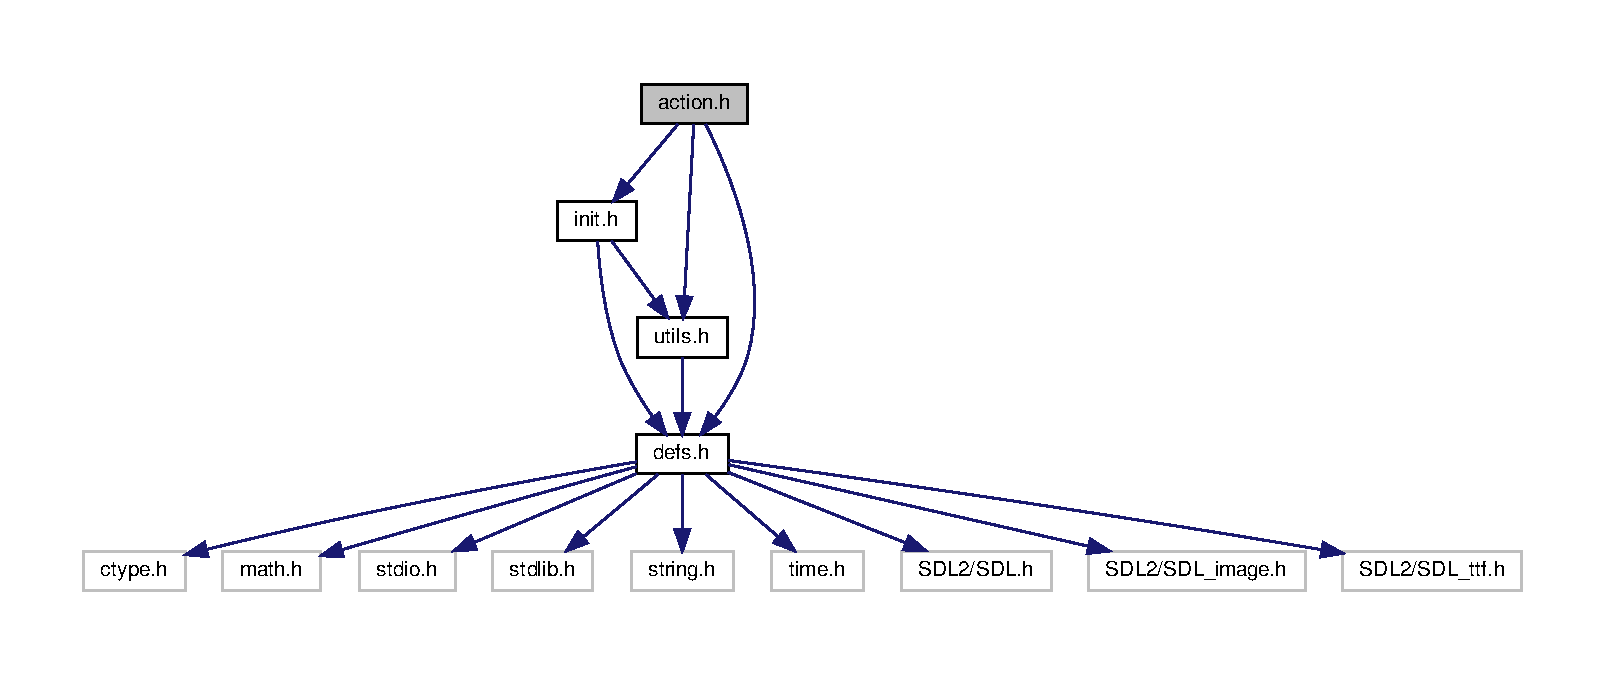
\includegraphics[width=350pt]{action_8h__incl}
\end{center}
\end{figure}
This graph shows which files directly or indirectly include this file\+:
\nopagebreak
\begin{figure}[H]
\begin{center}
\leavevmode
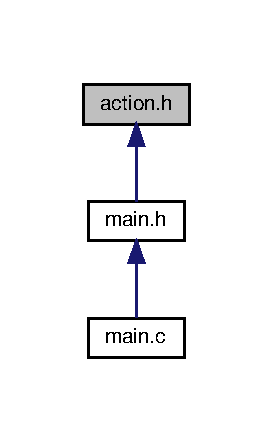
\includegraphics[width=131pt]{action_8h__dep__incl}
\end{center}
\end{figure}
\subsection*{Functions}
\begin{DoxyCompactItemize}
\item 
void \hyperlink{action_8h_a8738780a1642e9d07f6e89e5e48f647f}{Logic\+Game} (void)
\begin{DoxyCompactList}\small\item\em 게임 진행 중일 시 필요한 액션을 순차적으로 수행 \end{DoxyCompactList}\item 
void \hyperlink{action_8h_a582c79a5f61e7bf0a34e40fd59aa17c2}{Logic\+Game\+Over} (void)
\begin{DoxyCompactList}\small\item\em 게임오버된 상태에 필요한 액션을 순차적으로 수행 \end{DoxyCompactList}\item 
void \hyperlink{action_8h_ad1c341bd8d66cfa6307f9eda7fcb517f}{Act\+Player} (void)
\begin{DoxyCompactList}\small\item\em 키보드 입력 상태에 따라 주인공의 액션을 수행. 누른 화살표 버튼에 따라 움직이고, 화면 밖으로 나갈 수 없음. \end{DoxyCompactList}\item 
void \hyperlink{action_8h_a94b64a686b9deac756fc84a1f21d182a}{Act\+Bullet} (void)
\begin{DoxyCompactList}\small\item\em 총알의 액션을 수행. 주인공이 있는 방향으로 랜덤하게 날아가고, 화면 밖으로 나가면 리스폰됨. \end{DoxyCompactList}\item 
void \hyperlink{action_8h_a7d7e08b4f43179e1c112660ebf499f38}{Act\+Score\+Board} (void)
\begin{DoxyCompactList}\small\item\em 스코어보드 문자열 생성 (전역변수 score에 따라 현재 점수 표시) \end{DoxyCompactList}\item 
void \hyperlink{action_8h_aa65db23b8a8d08fdab84f41d2d77fc16}{Act\+Final\+Score\+Board} (void)
\begin{DoxyCompactList}\small\item\em 게임 오버 시 최종 스코어 문자열 생성 (전역변수 score에 따라 최종 점수 표시) \end{DoxyCompactList}\item 
void \hyperlink{action_8h_a95ce7534309c25f41e7f6c95a84526fe}{Act\+Check\+Death} (void)
\begin{DoxyCompactList}\small\item\em 총알과 주인공의 충돌 여부를 계산하고 충돌 시 게임 오버시킴 \end{DoxyCompactList}\item 
void \hyperlink{action_8h_a981d44fa9ea88e54c20d6a74c037277d}{Act\+Game\+Over} (void)
\begin{DoxyCompactList}\small\item\em 게임 오버 화면의 액션 수행. 아무 것도 수행하지 않다가, R키를 누르면 모든 구조체 초기화 \end{DoxyCompactList}\end{DoxyCompactItemize}
\subsection*{Variables}
\begin{DoxyCompactItemize}
\item 
\hyperlink{struct_app}{App} \hyperlink{action_8h_a05b5a24325d46227633053ca49de6234}{app}
\item 
\hyperlink{struct_entity}{Entity} \hyperlink{action_8h_aa98761129f4d5e69468dcbdddbd88d9d}{player}
\item 
\hyperlink{struct_entity}{Entity} \hyperlink{action_8h_a3969fcbadddf924ee352d7e232919bf5}{bullet} \mbox{[}\hyperlink{defs_8h_ac2f0ab514de41108a223c4edd49a6dfb}{N\+U\+M\+\_\+\+B\+U\+L\+L\+E\+TS}\mbox{]}
\item 
\hyperlink{struct_entity}{Entity} \hyperlink{action_8h_a30f03aaf13c260e57b759c650c99468e}{game\+\_\+over}
\item 
\hyperlink{struct_text}{Text} \hyperlink{action_8h_afef3fdea043a22bb19f93f3799421010}{score\+\_\+board}
\item 
char \hyperlink{action_8h_ae3c21975ce19d3b28f11d50419e15ab9}{score\+\_\+text} \mbox{[}\hyperlink{defs_8h_aeca034f67218340ecb2261a22c2f3dcd}{B\+U\+F\+S\+I\+ZE}\mbox{]}
\item 
int \hyperlink{action_8h_aef160b7437d94056f1dc59646cd5b87d}{score}
\end{DoxyCompactItemize}


\subsection{Detailed Description}
키보드 입력, 현재 주인공 및 총알의 상태를 바탕으로 액션을 수행하는 함수 선언 

\begin{DoxyAuthor}{Author}
이성재 (\href{mailto:seongjae.lee.1118@gmail.com}{\tt seongjae.\+lee.\+1118@gmail.\+com}) 
\end{DoxyAuthor}


\subsection{Function Documentation}
\mbox{\Hypertarget{action_8h_a94b64a686b9deac756fc84a1f21d182a}\label{action_8h_a94b64a686b9deac756fc84a1f21d182a}} 
\index{action.\+h@{action.\+h}!Act\+Bullet@{Act\+Bullet}}
\index{Act\+Bullet@{Act\+Bullet}!action.\+h@{action.\+h}}
\subsubsection{\texorpdfstring{Act\+Bullet()}{ActBullet()}}
{\footnotesize\ttfamily void Act\+Bullet (\begin{DoxyParamCaption}\item[{void}]{ }\end{DoxyParamCaption})}



총알의 액션을 수행. 주인공이 있는 방향으로 랜덤하게 날아가고, 화면 밖으로 나가면 리스폰됨. 

\begin{DoxyReturn}{Returns}
리턴 값 없음 
\end{DoxyReturn}
\mbox{\Hypertarget{action_8h_a95ce7534309c25f41e7f6c95a84526fe}\label{action_8h_a95ce7534309c25f41e7f6c95a84526fe}} 
\index{action.\+h@{action.\+h}!Act\+Check\+Death@{Act\+Check\+Death}}
\index{Act\+Check\+Death@{Act\+Check\+Death}!action.\+h@{action.\+h}}
\subsubsection{\texorpdfstring{Act\+Check\+Death()}{ActCheckDeath()}}
{\footnotesize\ttfamily void Act\+Check\+Death (\begin{DoxyParamCaption}\item[{void}]{ }\end{DoxyParamCaption})}



총알과 주인공의 충돌 여부를 계산하고 충돌 시 게임 오버시킴 

\begin{DoxyReturn}{Returns}
리턴 값 없음 
\end{DoxyReturn}
\mbox{\Hypertarget{action_8h_aa65db23b8a8d08fdab84f41d2d77fc16}\label{action_8h_aa65db23b8a8d08fdab84f41d2d77fc16}} 
\index{action.\+h@{action.\+h}!Act\+Final\+Score\+Board@{Act\+Final\+Score\+Board}}
\index{Act\+Final\+Score\+Board@{Act\+Final\+Score\+Board}!action.\+h@{action.\+h}}
\subsubsection{\texorpdfstring{Act\+Final\+Score\+Board()}{ActFinalScoreBoard()}}
{\footnotesize\ttfamily void Act\+Final\+Score\+Board (\begin{DoxyParamCaption}\item[{void}]{ }\end{DoxyParamCaption})}



게임 오버 시 최종 스코어 문자열 생성 (전역변수 score에 따라 최종 점수 표시) 

\begin{DoxyReturn}{Returns}
리턴 값 없음 
\end{DoxyReturn}
\mbox{\Hypertarget{action_8h_a981d44fa9ea88e54c20d6a74c037277d}\label{action_8h_a981d44fa9ea88e54c20d6a74c037277d}} 
\index{action.\+h@{action.\+h}!Act\+Game\+Over@{Act\+Game\+Over}}
\index{Act\+Game\+Over@{Act\+Game\+Over}!action.\+h@{action.\+h}}
\subsubsection{\texorpdfstring{Act\+Game\+Over()}{ActGameOver()}}
{\footnotesize\ttfamily void Act\+Game\+Over (\begin{DoxyParamCaption}\item[{void}]{ }\end{DoxyParamCaption})}



게임 오버 화면의 액션 수행. 아무 것도 수행하지 않다가, R키를 누르면 모든 구조체 초기화 

\begin{DoxyReturn}{Returns}
리턴 값 없음 
\end{DoxyReturn}
\mbox{\Hypertarget{action_8h_ad1c341bd8d66cfa6307f9eda7fcb517f}\label{action_8h_ad1c341bd8d66cfa6307f9eda7fcb517f}} 
\index{action.\+h@{action.\+h}!Act\+Player@{Act\+Player}}
\index{Act\+Player@{Act\+Player}!action.\+h@{action.\+h}}
\subsubsection{\texorpdfstring{Act\+Player()}{ActPlayer()}}
{\footnotesize\ttfamily void Act\+Player (\begin{DoxyParamCaption}\item[{void}]{ }\end{DoxyParamCaption})}



키보드 입력 상태에 따라 주인공의 액션을 수행. 누른 화살표 버튼에 따라 움직이고, 화면 밖으로 나갈 수 없음. 

\begin{DoxyReturn}{Returns}
리턴 값 없음 
\end{DoxyReturn}
\mbox{\Hypertarget{action_8h_a7d7e08b4f43179e1c112660ebf499f38}\label{action_8h_a7d7e08b4f43179e1c112660ebf499f38}} 
\index{action.\+h@{action.\+h}!Act\+Score\+Board@{Act\+Score\+Board}}
\index{Act\+Score\+Board@{Act\+Score\+Board}!action.\+h@{action.\+h}}
\subsubsection{\texorpdfstring{Act\+Score\+Board()}{ActScoreBoard()}}
{\footnotesize\ttfamily void Act\+Score\+Board (\begin{DoxyParamCaption}\item[{void}]{ }\end{DoxyParamCaption})}



스코어보드 문자열 생성 (전역변수 score에 따라 현재 점수 표시) 

\begin{DoxyReturn}{Returns}
리턴 값 없음 
\end{DoxyReturn}
\mbox{\Hypertarget{action_8h_a8738780a1642e9d07f6e89e5e48f647f}\label{action_8h_a8738780a1642e9d07f6e89e5e48f647f}} 
\index{action.\+h@{action.\+h}!Logic\+Game@{Logic\+Game}}
\index{Logic\+Game@{Logic\+Game}!action.\+h@{action.\+h}}
\subsubsection{\texorpdfstring{Logic\+Game()}{LogicGame()}}
{\footnotesize\ttfamily void Logic\+Game (\begin{DoxyParamCaption}\item[{void}]{ }\end{DoxyParamCaption})}



게임 진행 중일 시 필요한 액션을 순차적으로 수행 

\begin{DoxyReturn}{Returns}
리턴 값 없음 
\end{DoxyReturn}
\mbox{\Hypertarget{action_8h_a582c79a5f61e7bf0a34e40fd59aa17c2}\label{action_8h_a582c79a5f61e7bf0a34e40fd59aa17c2}} 
\index{action.\+h@{action.\+h}!Logic\+Game\+Over@{Logic\+Game\+Over}}
\index{Logic\+Game\+Over@{Logic\+Game\+Over}!action.\+h@{action.\+h}}
\subsubsection{\texorpdfstring{Logic\+Game\+Over()}{LogicGameOver()}}
{\footnotesize\ttfamily void Logic\+Game\+Over (\begin{DoxyParamCaption}\item[{void}]{ }\end{DoxyParamCaption})}



게임오버된 상태에 필요한 액션을 순차적으로 수행 

\begin{DoxyReturn}{Returns}
리턴 값 없음 
\end{DoxyReturn}


\subsection{Variable Documentation}
\mbox{\Hypertarget{action_8h_a05b5a24325d46227633053ca49de6234}\label{action_8h_a05b5a24325d46227633053ca49de6234}} 
\index{action.\+h@{action.\+h}!app@{app}}
\index{app@{app}!action.\+h@{action.\+h}}
\subsubsection{\texorpdfstring{app}{app}}
{\footnotesize\ttfamily \hyperlink{struct_app}{App} app}

프로그램 전체 단위로 관리하는 전역 객체 모음 \mbox{\Hypertarget{action_8h_a3969fcbadddf924ee352d7e232919bf5}\label{action_8h_a3969fcbadddf924ee352d7e232919bf5}} 
\index{action.\+h@{action.\+h}!bullet@{bullet}}
\index{bullet@{bullet}!action.\+h@{action.\+h}}
\subsubsection{\texorpdfstring{bullet}{bullet}}
{\footnotesize\ttfamily \hyperlink{struct_entity}{Entity} bullet\mbox{[}\hyperlink{defs_8h_ac2f0ab514de41108a223c4edd49a6dfb}{N\+U\+M\+\_\+\+B\+U\+L\+L\+E\+TS}\mbox{]}}

총알의 속성을 설명하는 Entity형 구조체 \mbox{\Hypertarget{action_8h_a30f03aaf13c260e57b759c650c99468e}\label{action_8h_a30f03aaf13c260e57b759c650c99468e}} 
\index{action.\+h@{action.\+h}!game\+\_\+over@{game\+\_\+over}}
\index{game\+\_\+over@{game\+\_\+over}!action.\+h@{action.\+h}}
\subsubsection{\texorpdfstring{game\+\_\+over}{game\_over}}
{\footnotesize\ttfamily \hyperlink{struct_entity}{Entity} game\+\_\+over}

게임오버 화면의 속성을 설명하는 Entity형 구조체 \mbox{\Hypertarget{action_8h_aa98761129f4d5e69468dcbdddbd88d9d}\label{action_8h_aa98761129f4d5e69468dcbdddbd88d9d}} 
\index{action.\+h@{action.\+h}!player@{player}}
\index{player@{player}!action.\+h@{action.\+h}}
\subsubsection{\texorpdfstring{player}{player}}
{\footnotesize\ttfamily \hyperlink{struct_entity}{Entity} player}

주인공의 속성을 설명하는 Entity형 구조체 \mbox{\Hypertarget{action_8h_aef160b7437d94056f1dc59646cd5b87d}\label{action_8h_aef160b7437d94056f1dc59646cd5b87d}} 
\index{action.\+h@{action.\+h}!score@{score}}
\index{score@{score}!action.\+h@{action.\+h}}
\subsubsection{\texorpdfstring{score}{score}}
{\footnotesize\ttfamily int score}

게임 스코어 \mbox{\Hypertarget{action_8h_afef3fdea043a22bb19f93f3799421010}\label{action_8h_afef3fdea043a22bb19f93f3799421010}} 
\index{action.\+h@{action.\+h}!score\+\_\+board@{score\+\_\+board}}
\index{score\+\_\+board@{score\+\_\+board}!action.\+h@{action.\+h}}
\subsubsection{\texorpdfstring{score\+\_\+board}{score\_board}}
{\footnotesize\ttfamily \hyperlink{struct_text}{Text} score\+\_\+board}

우상단 스코어보드 문자열을 설명하는 Text형 구조체 \mbox{\Hypertarget{action_8h_ae3c21975ce19d3b28f11d50419e15ab9}\label{action_8h_ae3c21975ce19d3b28f11d50419e15ab9}} 
\index{action.\+h@{action.\+h}!score\+\_\+text@{score\+\_\+text}}
\index{score\+\_\+text@{score\+\_\+text}!action.\+h@{action.\+h}}
\subsubsection{\texorpdfstring{score\+\_\+text}{score\_text}}
{\footnotesize\ttfamily char score\+\_\+text\mbox{[}\hyperlink{defs_8h_aeca034f67218340ecb2261a22c2f3dcd}{B\+U\+F\+S\+I\+ZE}\mbox{]}}

스코어보드에 출력할 문자열 
\hypertarget{defs_8h}{}\section{defs.\+h File Reference}
\label{defs_8h}\index{defs.\+h@{defs.\+h}}


데이터타입 및 상수 정의  


{\ttfamily \#include \char`\"{}ctype.\+h\char`\"{}}\newline
{\ttfamily \#include \char`\"{}math.\+h\char`\"{}}\newline
{\ttfamily \#include \char`\"{}stdio.\+h\char`\"{}}\newline
{\ttfamily \#include \char`\"{}stdlib.\+h\char`\"{}}\newline
{\ttfamily \#include \char`\"{}string.\+h\char`\"{}}\newline
{\ttfamily \#include \char`\"{}time.\+h\char`\"{}}\newline
{\ttfamily \#include \char`\"{}S\+D\+L2/\+S\+D\+L.\+h\char`\"{}}\newline
{\ttfamily \#include \char`\"{}S\+D\+L2/\+S\+D\+L\+\_\+image.\+h\char`\"{}}\newline
{\ttfamily \#include \char`\"{}S\+D\+L2/\+S\+D\+L\+\_\+ttf.\+h\char`\"{}}\newline
Include dependency graph for defs.\+h\+:
\nopagebreak
\begin{figure}[H]
\begin{center}
\leavevmode
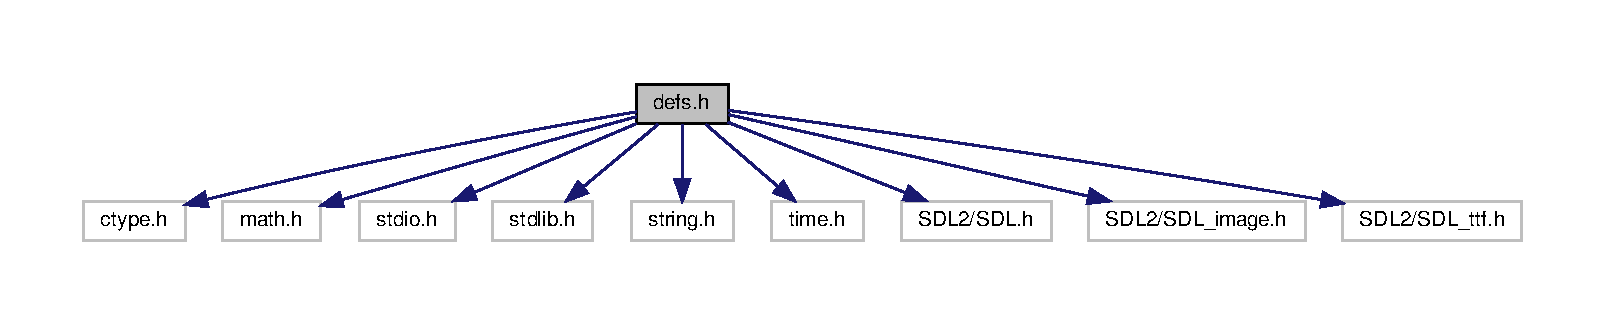
\includegraphics[width=350pt]{defs_8h__incl}
\end{center}
\end{figure}
This graph shows which files directly or indirectly include this file\+:
\nopagebreak
\begin{figure}[H]
\begin{center}
\leavevmode
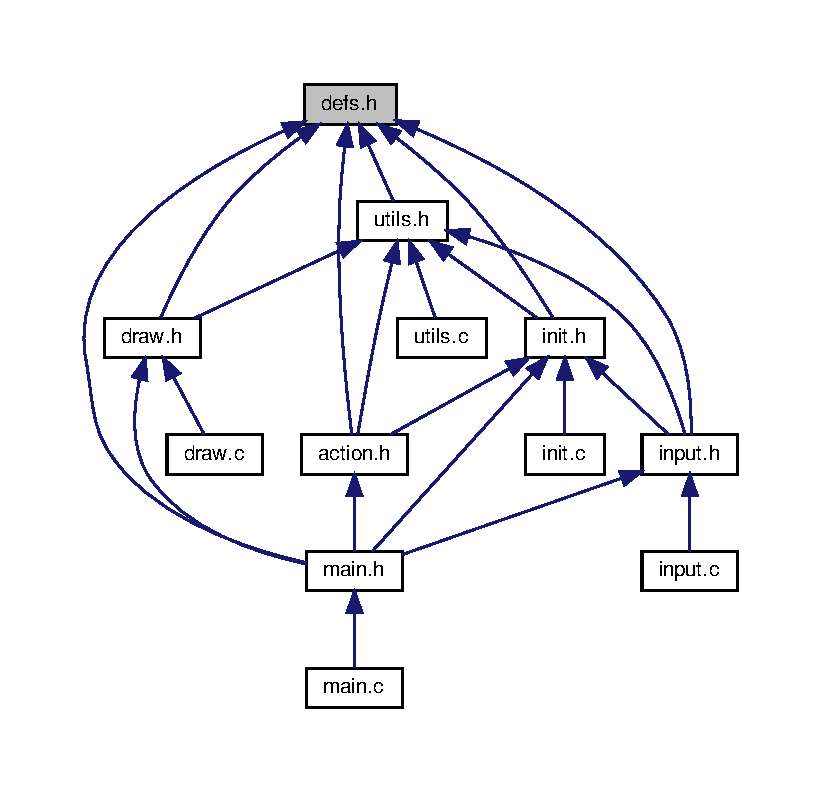
\includegraphics[width=350pt]{defs_8h__dep__incl}
\end{center}
\end{figure}
\subsection*{Classes}
\begin{DoxyCompactItemize}
\item 
struct \hyperlink{struct_app}{App}
\begin{DoxyCompactList}\small\item\em \hyperlink{struct_app}{App}\+: 프로그램 전체적으로 관리해야 하는 요소를 모아 놓은 구조체 \end{DoxyCompactList}\item 
struct \hyperlink{struct_entity}{Entity}
\begin{DoxyCompactList}\small\item\em \hyperlink{struct_entity}{Entity}\+: 게임 내에서 움직이는 물체를 구현하기 위한 구조체(주인공, 총알) \end{DoxyCompactList}\item 
struct \hyperlink{struct_text}{Text}
\begin{DoxyCompactList}\small\item\em \hyperlink{struct_text}{Text}\+: 게임 내에 문자열을 표시할 경우 문자열을 나타내는 구조체(스코어보드) \end{DoxyCompactList}\end{DoxyCompactItemize}
\subsection*{Macros}
\begin{DoxyCompactItemize}
\item 
\#define \hyperlink{defs_8h_ac92ca5ab87034a348decad7ee8d4bd1b}{F\+PS}~60
\item 
\#define \hyperlink{defs_8h_aeca034f67218340ecb2261a22c2f3dcd}{B\+U\+F\+S\+I\+ZE}~1024
\item 
\#define \hyperlink{defs_8h_a2cd109632a6dcccaa80b43561b1ab700}{S\+C\+R\+E\+E\+N\+\_\+\+W\+I\+D\+TH}~640
\item 
\#define \hyperlink{defs_8h_a6974d08a74da681b3957b2fead2608b8}{S\+C\+R\+E\+E\+N\+\_\+\+H\+E\+I\+G\+HT}~480
\item 
\#define \hyperlink{defs_8h_a89e2ac9092225702ac543695d0771d38}{P\+L\+A\+Y\+E\+R\+\_\+\+W\+I\+D\+TH}~24
\item 
\#define \hyperlink{defs_8h_a2712b06fd52f25adca031d05c3e0c09b}{P\+L\+A\+Y\+E\+R\+\_\+\+H\+E\+I\+G\+HT}~24
\item 
\#define \hyperlink{defs_8h_af49bad41acef45feb40939c0cf9d5d35}{P\+L\+A\+Y\+E\+R\+\_\+\+S\+P\+E\+ED}~4
\item 
\#define \hyperlink{defs_8h_ad135231941b972722b6ef5f5bd0670d2}{B\+U\+L\+L\+E\+T\+\_\+\+W\+I\+D\+TH}~8
\item 
\#define \hyperlink{defs_8h_ac91cd0386a836b604804b5dd09c0a65c}{B\+U\+L\+L\+E\+T\+\_\+\+H\+E\+I\+G\+HT}~8
\item 
\#define \hyperlink{defs_8h_a70b3e643b533b8f785b7912e69434161}{B\+U\+L\+L\+E\+T\+\_\+\+S\+P\+E\+ED}~6
\item 
\#define \hyperlink{defs_8h_ac2f0ab514de41108a223c4edd49a6dfb}{N\+U\+M\+\_\+\+B\+U\+L\+L\+E\+TS}~16
\item 
\#define \hyperlink{defs_8h_a5d52eeb41a03aeda6974d60772531f96}{F\+O\+N\+T\+S\+I\+ZE}~20
\end{DoxyCompactItemize}


\subsection{Detailed Description}
데이터타입 및 상수 정의 

\begin{DoxyAuthor}{Author}
이성재 (\href{mailto:seongjae.lee.1118@gmail.com}{\tt seongjae.\+lee.\+1118@gmail.\+com}) 
\end{DoxyAuthor}


\subsection{Macro Definition Documentation}
\mbox{\Hypertarget{defs_8h_aeca034f67218340ecb2261a22c2f3dcd}\label{defs_8h_aeca034f67218340ecb2261a22c2f3dcd}} 
\index{defs.\+h@{defs.\+h}!B\+U\+F\+S\+I\+ZE@{B\+U\+F\+S\+I\+ZE}}
\index{B\+U\+F\+S\+I\+ZE@{B\+U\+F\+S\+I\+ZE}!defs.\+h@{defs.\+h}}
\subsubsection{\texorpdfstring{B\+U\+F\+S\+I\+ZE}{BUFSIZE}}
{\footnotesize\ttfamily \#define B\+U\+F\+S\+I\+ZE~1024}

문자열 버퍼 크기 \mbox{\Hypertarget{defs_8h_ac91cd0386a836b604804b5dd09c0a65c}\label{defs_8h_ac91cd0386a836b604804b5dd09c0a65c}} 
\index{defs.\+h@{defs.\+h}!B\+U\+L\+L\+E\+T\+\_\+\+H\+E\+I\+G\+HT@{B\+U\+L\+L\+E\+T\+\_\+\+H\+E\+I\+G\+HT}}
\index{B\+U\+L\+L\+E\+T\+\_\+\+H\+E\+I\+G\+HT@{B\+U\+L\+L\+E\+T\+\_\+\+H\+E\+I\+G\+HT}!defs.\+h@{defs.\+h}}
\subsubsection{\texorpdfstring{B\+U\+L\+L\+E\+T\+\_\+\+H\+E\+I\+G\+HT}{BULLET\_HEIGHT}}
{\footnotesize\ttfamily \#define B\+U\+L\+L\+E\+T\+\_\+\+H\+E\+I\+G\+HT~8}

총알 객체 높이(픽셀) \mbox{\Hypertarget{defs_8h_a70b3e643b533b8f785b7912e69434161}\label{defs_8h_a70b3e643b533b8f785b7912e69434161}} 
\index{defs.\+h@{defs.\+h}!B\+U\+L\+L\+E\+T\+\_\+\+S\+P\+E\+ED@{B\+U\+L\+L\+E\+T\+\_\+\+S\+P\+E\+ED}}
\index{B\+U\+L\+L\+E\+T\+\_\+\+S\+P\+E\+ED@{B\+U\+L\+L\+E\+T\+\_\+\+S\+P\+E\+ED}!defs.\+h@{defs.\+h}}
\subsubsection{\texorpdfstring{B\+U\+L\+L\+E\+T\+\_\+\+S\+P\+E\+ED}{BULLET\_SPEED}}
{\footnotesize\ttfamily \#define B\+U\+L\+L\+E\+T\+\_\+\+S\+P\+E\+ED~6}

총알 객체 속도(단위시간당 이동량) \mbox{\Hypertarget{defs_8h_ad135231941b972722b6ef5f5bd0670d2}\label{defs_8h_ad135231941b972722b6ef5f5bd0670d2}} 
\index{defs.\+h@{defs.\+h}!B\+U\+L\+L\+E\+T\+\_\+\+W\+I\+D\+TH@{B\+U\+L\+L\+E\+T\+\_\+\+W\+I\+D\+TH}}
\index{B\+U\+L\+L\+E\+T\+\_\+\+W\+I\+D\+TH@{B\+U\+L\+L\+E\+T\+\_\+\+W\+I\+D\+TH}!defs.\+h@{defs.\+h}}
\subsubsection{\texorpdfstring{B\+U\+L\+L\+E\+T\+\_\+\+W\+I\+D\+TH}{BULLET\_WIDTH}}
{\footnotesize\ttfamily \#define B\+U\+L\+L\+E\+T\+\_\+\+W\+I\+D\+TH~8}

총알 객체 너비(픽셀) \mbox{\Hypertarget{defs_8h_a5d52eeb41a03aeda6974d60772531f96}\label{defs_8h_a5d52eeb41a03aeda6974d60772531f96}} 
\index{defs.\+h@{defs.\+h}!F\+O\+N\+T\+S\+I\+ZE@{F\+O\+N\+T\+S\+I\+ZE}}
\index{F\+O\+N\+T\+S\+I\+ZE@{F\+O\+N\+T\+S\+I\+ZE}!defs.\+h@{defs.\+h}}
\subsubsection{\texorpdfstring{F\+O\+N\+T\+S\+I\+ZE}{FONTSIZE}}
{\footnotesize\ttfamily \#define F\+O\+N\+T\+S\+I\+ZE~20}

출력할 문자열 폰트 크기 \mbox{\Hypertarget{defs_8h_ac92ca5ab87034a348decad7ee8d4bd1b}\label{defs_8h_ac92ca5ab87034a348decad7ee8d4bd1b}} 
\index{defs.\+h@{defs.\+h}!F\+PS@{F\+PS}}
\index{F\+PS@{F\+PS}!defs.\+h@{defs.\+h}}
\subsubsection{\texorpdfstring{F\+PS}{FPS}}
{\footnotesize\ttfamily \#define F\+PS~60}

게임 F\+PS \mbox{\Hypertarget{defs_8h_ac2f0ab514de41108a223c4edd49a6dfb}\label{defs_8h_ac2f0ab514de41108a223c4edd49a6dfb}} 
\index{defs.\+h@{defs.\+h}!N\+U\+M\+\_\+\+B\+U\+L\+L\+E\+TS@{N\+U\+M\+\_\+\+B\+U\+L\+L\+E\+TS}}
\index{N\+U\+M\+\_\+\+B\+U\+L\+L\+E\+TS@{N\+U\+M\+\_\+\+B\+U\+L\+L\+E\+TS}!defs.\+h@{defs.\+h}}
\subsubsection{\texorpdfstring{N\+U\+M\+\_\+\+B\+U\+L\+L\+E\+TS}{NUM\_BULLETS}}
{\footnotesize\ttfamily \#define N\+U\+M\+\_\+\+B\+U\+L\+L\+E\+TS~16}

총알 전체 갯수 \mbox{\Hypertarget{defs_8h_a2712b06fd52f25adca031d05c3e0c09b}\label{defs_8h_a2712b06fd52f25adca031d05c3e0c09b}} 
\index{defs.\+h@{defs.\+h}!P\+L\+A\+Y\+E\+R\+\_\+\+H\+E\+I\+G\+HT@{P\+L\+A\+Y\+E\+R\+\_\+\+H\+E\+I\+G\+HT}}
\index{P\+L\+A\+Y\+E\+R\+\_\+\+H\+E\+I\+G\+HT@{P\+L\+A\+Y\+E\+R\+\_\+\+H\+E\+I\+G\+HT}!defs.\+h@{defs.\+h}}
\subsubsection{\texorpdfstring{P\+L\+A\+Y\+E\+R\+\_\+\+H\+E\+I\+G\+HT}{PLAYER\_HEIGHT}}
{\footnotesize\ttfamily \#define P\+L\+A\+Y\+E\+R\+\_\+\+H\+E\+I\+G\+HT~24}

플레이어 객체 높이(픽셀) \mbox{\Hypertarget{defs_8h_af49bad41acef45feb40939c0cf9d5d35}\label{defs_8h_af49bad41acef45feb40939c0cf9d5d35}} 
\index{defs.\+h@{defs.\+h}!P\+L\+A\+Y\+E\+R\+\_\+\+S\+P\+E\+ED@{P\+L\+A\+Y\+E\+R\+\_\+\+S\+P\+E\+ED}}
\index{P\+L\+A\+Y\+E\+R\+\_\+\+S\+P\+E\+ED@{P\+L\+A\+Y\+E\+R\+\_\+\+S\+P\+E\+ED}!defs.\+h@{defs.\+h}}
\subsubsection{\texorpdfstring{P\+L\+A\+Y\+E\+R\+\_\+\+S\+P\+E\+ED}{PLAYER\_SPEED}}
{\footnotesize\ttfamily \#define P\+L\+A\+Y\+E\+R\+\_\+\+S\+P\+E\+ED~4}

플레이어 객체 속도(단위시간당 이동량) \mbox{\Hypertarget{defs_8h_a89e2ac9092225702ac543695d0771d38}\label{defs_8h_a89e2ac9092225702ac543695d0771d38}} 
\index{defs.\+h@{defs.\+h}!P\+L\+A\+Y\+E\+R\+\_\+\+W\+I\+D\+TH@{P\+L\+A\+Y\+E\+R\+\_\+\+W\+I\+D\+TH}}
\index{P\+L\+A\+Y\+E\+R\+\_\+\+W\+I\+D\+TH@{P\+L\+A\+Y\+E\+R\+\_\+\+W\+I\+D\+TH}!defs.\+h@{defs.\+h}}
\subsubsection{\texorpdfstring{P\+L\+A\+Y\+E\+R\+\_\+\+W\+I\+D\+TH}{PLAYER\_WIDTH}}
{\footnotesize\ttfamily \#define P\+L\+A\+Y\+E\+R\+\_\+\+W\+I\+D\+TH~24}

플레이어 객체 너비(픽셀) \mbox{\Hypertarget{defs_8h_a6974d08a74da681b3957b2fead2608b8}\label{defs_8h_a6974d08a74da681b3957b2fead2608b8}} 
\index{defs.\+h@{defs.\+h}!S\+C\+R\+E\+E\+N\+\_\+\+H\+E\+I\+G\+HT@{S\+C\+R\+E\+E\+N\+\_\+\+H\+E\+I\+G\+HT}}
\index{S\+C\+R\+E\+E\+N\+\_\+\+H\+E\+I\+G\+HT@{S\+C\+R\+E\+E\+N\+\_\+\+H\+E\+I\+G\+HT}!defs.\+h@{defs.\+h}}
\subsubsection{\texorpdfstring{S\+C\+R\+E\+E\+N\+\_\+\+H\+E\+I\+G\+HT}{SCREEN\_HEIGHT}}
{\footnotesize\ttfamily \#define S\+C\+R\+E\+E\+N\+\_\+\+H\+E\+I\+G\+HT~480}

화면 높이(픽셀) \mbox{\Hypertarget{defs_8h_a2cd109632a6dcccaa80b43561b1ab700}\label{defs_8h_a2cd109632a6dcccaa80b43561b1ab700}} 
\index{defs.\+h@{defs.\+h}!S\+C\+R\+E\+E\+N\+\_\+\+W\+I\+D\+TH@{S\+C\+R\+E\+E\+N\+\_\+\+W\+I\+D\+TH}}
\index{S\+C\+R\+E\+E\+N\+\_\+\+W\+I\+D\+TH@{S\+C\+R\+E\+E\+N\+\_\+\+W\+I\+D\+TH}!defs.\+h@{defs.\+h}}
\subsubsection{\texorpdfstring{S\+C\+R\+E\+E\+N\+\_\+\+W\+I\+D\+TH}{SCREEN\_WIDTH}}
{\footnotesize\ttfamily \#define S\+C\+R\+E\+E\+N\+\_\+\+W\+I\+D\+TH~640}

화면 너비(픽셀) 
\hypertarget{draw_8c}{}\section{draw.\+c File Reference}
\label{draw_8c}\index{draw.\+c@{draw.\+c}}


텍스쳐 렌더링을 수행하는 함수 정의  


{\ttfamily \#include \char`\"{}draw.\+h\char`\"{}}\newline
Include dependency graph for draw.\+c\+:
\nopagebreak
\begin{figure}[H]
\begin{center}
\leavevmode
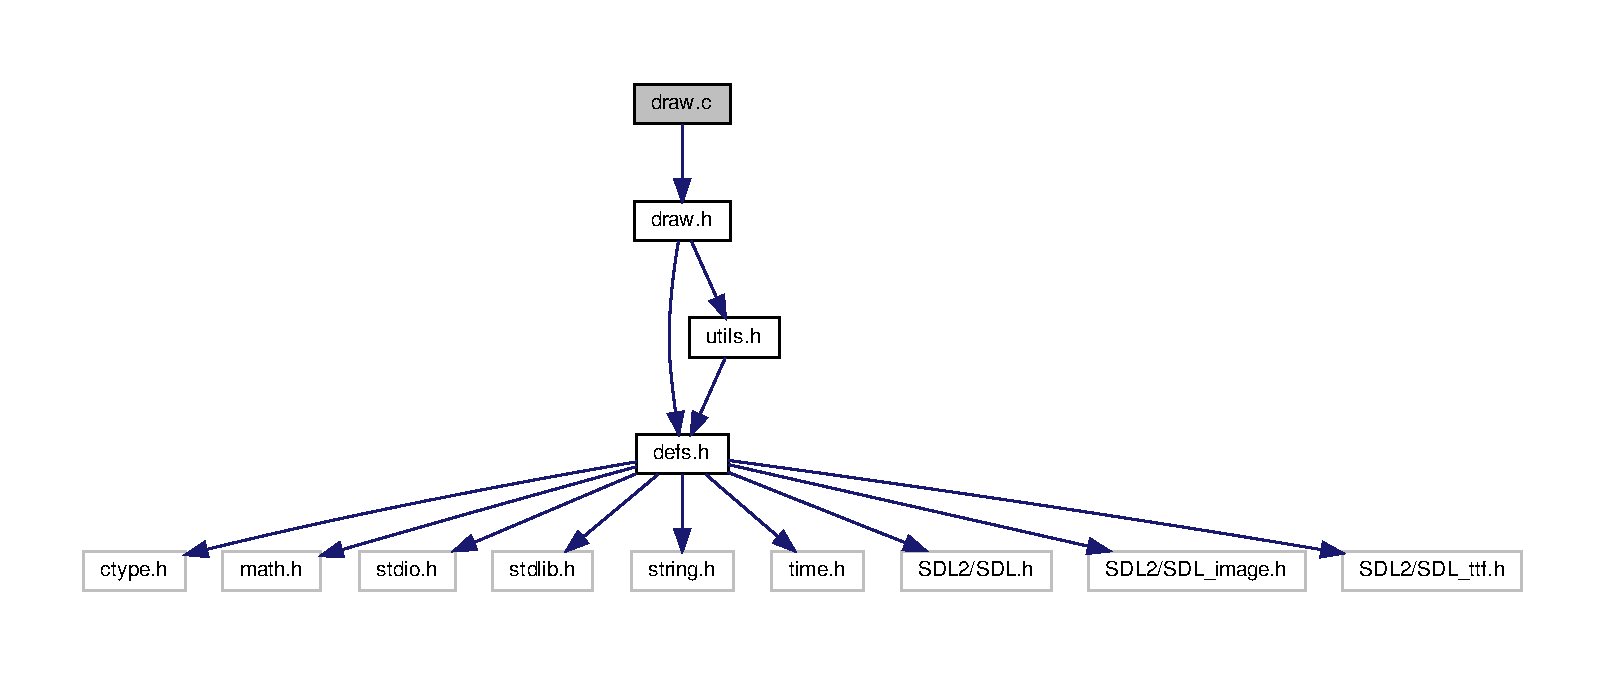
\includegraphics[width=350pt]{draw_8c__incl}
\end{center}
\end{figure}
\subsection*{Functions}
\begin{DoxyCompactItemize}
\item 
void \hyperlink{draw_8c_a07863ec93360df2f9a1b5eff97890563}{Clear\+Window} (void)
\begin{DoxyCompactList}\small\item\em 배경을 흰색으로 지정하고 화면에 렌더링된 모든 요소 제거 \end{DoxyCompactList}\item 
void \hyperlink{draw_8c_a17ef8abf91a443ec16525f4d95d7836e}{Show\+Window} (void)
\begin{DoxyCompactList}\small\item\em 화면에 렌더링 결과 표시(보여주기) \end{DoxyCompactList}\item 
void \hyperlink{draw_8c_ab33f4146ab23c4be91566a68e68895fe}{Draw\+Game} (void)
\begin{DoxyCompactList}\small\item\em 게임 진행 상태에서 주인공, 총알, 스코어보드 렌더링 \end{DoxyCompactList}\item 
void \hyperlink{draw_8c_a52d7bd7319e47472de78cdbf95856b88}{Draw\+Game\+Over} (void)
\begin{DoxyCompactList}\small\item\em 게임 오버 상태에서 게임 오버 화면, 최종 스코어 렌더링 \end{DoxyCompactList}\item 
void \hyperlink{draw_8c_a303fcf31d5f32fbaa70040fa5848ff04}{Render\+Entity} (\hyperlink{struct_entity}{Entity} $\ast$object)
\begin{DoxyCompactList}\small\item\em \hyperlink{struct_entity}{Entity} 구조체 렌더링 \end{DoxyCompactList}\item 
void \hyperlink{draw_8c_a0e4dc5510d16de6f635e3229e999bddc}{Render\+Score\+Board} (\hyperlink{struct_text}{Text} $\ast$object)
\begin{DoxyCompactList}\small\item\em \hyperlink{struct_text}{Text} 구조체 렌더링 (스코어보드) \end{DoxyCompactList}\end{DoxyCompactItemize}


\subsection{Detailed Description}
텍스쳐 렌더링을 수행하는 함수 정의 

\begin{DoxyAuthor}{Author}
이성재 (\href{mailto:seongjae.lee.1118@gmail.com}{\tt seongjae.\+lee.\+1118@gmail.\+com}) 
\end{DoxyAuthor}


\subsection{Function Documentation}
\mbox{\Hypertarget{draw_8c_a07863ec93360df2f9a1b5eff97890563}\label{draw_8c_a07863ec93360df2f9a1b5eff97890563}} 
\index{draw.\+c@{draw.\+c}!Clear\+Window@{Clear\+Window}}
\index{Clear\+Window@{Clear\+Window}!draw.\+c@{draw.\+c}}
\subsubsection{\texorpdfstring{Clear\+Window()}{ClearWindow()}}
{\footnotesize\ttfamily void Clear\+Window (\begin{DoxyParamCaption}\item[{void}]{ }\end{DoxyParamCaption})}



배경을 흰색으로 지정하고 화면에 렌더링된 모든 요소 제거 

\begin{DoxyReturn}{Returns}
리턴 값 없음 
\end{DoxyReturn}
\mbox{\Hypertarget{draw_8c_ab33f4146ab23c4be91566a68e68895fe}\label{draw_8c_ab33f4146ab23c4be91566a68e68895fe}} 
\index{draw.\+c@{draw.\+c}!Draw\+Game@{Draw\+Game}}
\index{Draw\+Game@{Draw\+Game}!draw.\+c@{draw.\+c}}
\subsubsection{\texorpdfstring{Draw\+Game()}{DrawGame()}}
{\footnotesize\ttfamily void Draw\+Game (\begin{DoxyParamCaption}\item[{void}]{ }\end{DoxyParamCaption})}



게임 진행 상태에서 주인공, 총알, 스코어보드 렌더링 

\begin{DoxyReturn}{Returns}
리턴 값 없음 
\end{DoxyReturn}
\mbox{\Hypertarget{draw_8c_a52d7bd7319e47472de78cdbf95856b88}\label{draw_8c_a52d7bd7319e47472de78cdbf95856b88}} 
\index{draw.\+c@{draw.\+c}!Draw\+Game\+Over@{Draw\+Game\+Over}}
\index{Draw\+Game\+Over@{Draw\+Game\+Over}!draw.\+c@{draw.\+c}}
\subsubsection{\texorpdfstring{Draw\+Game\+Over()}{DrawGameOver()}}
{\footnotesize\ttfamily void Draw\+Game\+Over (\begin{DoxyParamCaption}\item[{void}]{ }\end{DoxyParamCaption})}



게임 오버 상태에서 게임 오버 화면, 최종 스코어 렌더링 

\begin{DoxyReturn}{Returns}
리턴 값 없음 
\end{DoxyReturn}
\mbox{\Hypertarget{draw_8c_a303fcf31d5f32fbaa70040fa5848ff04}\label{draw_8c_a303fcf31d5f32fbaa70040fa5848ff04}} 
\index{draw.\+c@{draw.\+c}!Render\+Entity@{Render\+Entity}}
\index{Render\+Entity@{Render\+Entity}!draw.\+c@{draw.\+c}}
\subsubsection{\texorpdfstring{Render\+Entity()}{RenderEntity()}}
{\footnotesize\ttfamily void Render\+Entity (\begin{DoxyParamCaption}\item[{\hyperlink{struct_entity}{Entity} $\ast$}]{object }\end{DoxyParamCaption})}



\hyperlink{struct_entity}{Entity} 구조체 렌더링 


\begin{DoxyParams}{Parameters}
{\em object} & 렌더링 대상 \hyperlink{struct_entity}{Entity} 구조체\\
\hline
\end{DoxyParams}
\begin{DoxyReturn}{Returns}
리턴 값 없음 
\end{DoxyReturn}
\mbox{\Hypertarget{draw_8c_a0e4dc5510d16de6f635e3229e999bddc}\label{draw_8c_a0e4dc5510d16de6f635e3229e999bddc}} 
\index{draw.\+c@{draw.\+c}!Render\+Score\+Board@{Render\+Score\+Board}}
\index{Render\+Score\+Board@{Render\+Score\+Board}!draw.\+c@{draw.\+c}}
\subsubsection{\texorpdfstring{Render\+Score\+Board()}{RenderScoreBoard()}}
{\footnotesize\ttfamily void Render\+Score\+Board (\begin{DoxyParamCaption}\item[{\hyperlink{struct_text}{Text} $\ast$}]{object }\end{DoxyParamCaption})}



\hyperlink{struct_text}{Text} 구조체 렌더링 (스코어보드) 


\begin{DoxyParams}{Parameters}
{\em object} & 렌더링 대상 \hyperlink{struct_text}{Text} 구조체\\
\hline
\end{DoxyParams}
\begin{DoxyReturn}{Returns}
리턴 값 없음 
\end{DoxyReturn}
\mbox{\Hypertarget{draw_8c_a17ef8abf91a443ec16525f4d95d7836e}\label{draw_8c_a17ef8abf91a443ec16525f4d95d7836e}} 
\index{draw.\+c@{draw.\+c}!Show\+Window@{Show\+Window}}
\index{Show\+Window@{Show\+Window}!draw.\+c@{draw.\+c}}
\subsubsection{\texorpdfstring{Show\+Window()}{ShowWindow()}}
{\footnotesize\ttfamily void Show\+Window (\begin{DoxyParamCaption}\item[{void}]{ }\end{DoxyParamCaption})}



화면에 렌더링 결과 표시(보여주기) 

\begin{DoxyReturn}{Returns}
리턴 값 없음 
\end{DoxyReturn}

\hypertarget{draw_8h}{}\section{draw.\+h File Reference}
\label{draw_8h}\index{draw.\+h@{draw.\+h}}


텍스쳐 렌더링을 수행하는 함수 선언  


{\ttfamily \#include \char`\"{}defs.\+h\char`\"{}}\newline
{\ttfamily \#include \char`\"{}utils.\+h\char`\"{}}\newline
Include dependency graph for draw.\+h\+:
\nopagebreak
\begin{figure}[H]
\begin{center}
\leavevmode
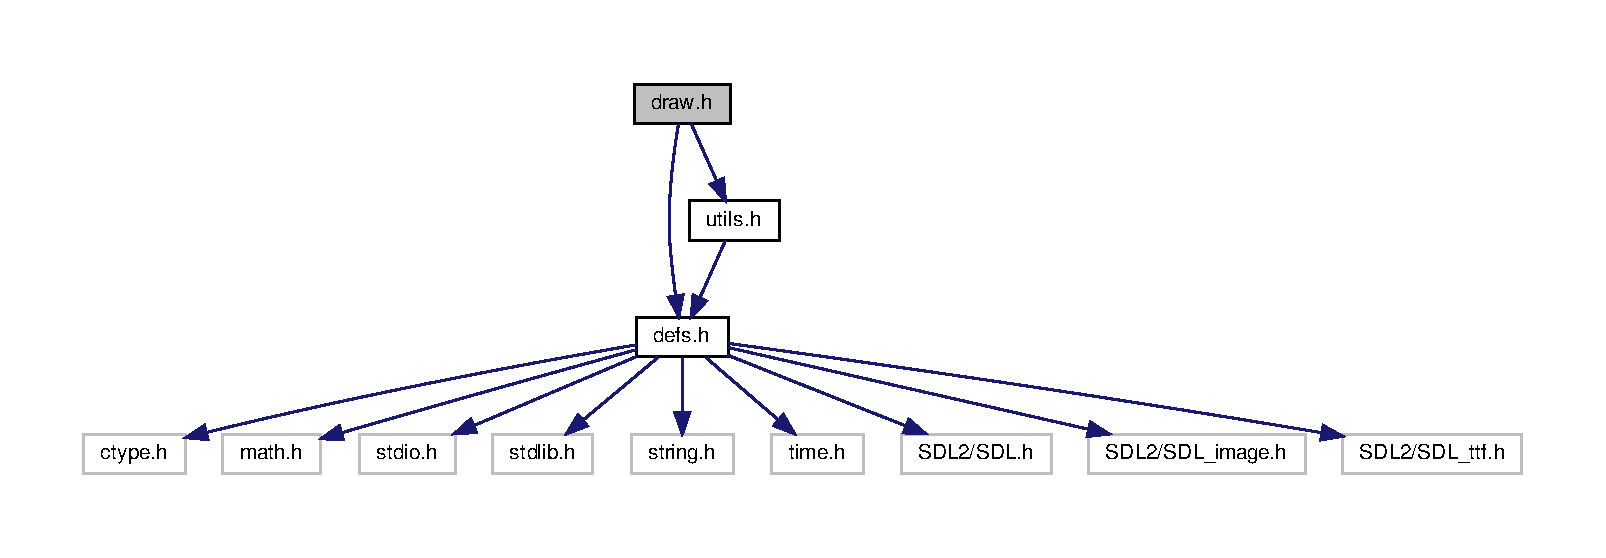
\includegraphics[width=350pt]{draw_8h__incl}
\end{center}
\end{figure}
This graph shows which files directly or indirectly include this file\+:
\nopagebreak
\begin{figure}[H]
\begin{center}
\leavevmode
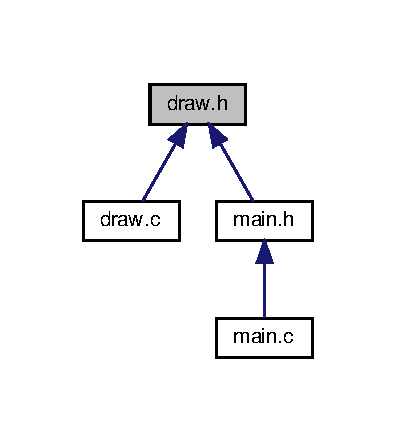
\includegraphics[width=190pt]{draw_8h__dep__incl}
\end{center}
\end{figure}
\subsection*{Functions}
\begin{DoxyCompactItemize}
\item 
void \hyperlink{draw_8h_a07863ec93360df2f9a1b5eff97890563}{Clear\+Window} (void)
\begin{DoxyCompactList}\small\item\em 배경을 흰색으로 지정하고 화면에 렌더링된 모든 요소 제거 \end{DoxyCompactList}\item 
void \hyperlink{draw_8h_a17ef8abf91a443ec16525f4d95d7836e}{Show\+Window} (void)
\begin{DoxyCompactList}\small\item\em 화면에 렌더링 결과 표시(보여주기) \end{DoxyCompactList}\item 
void \hyperlink{draw_8h_ab33f4146ab23c4be91566a68e68895fe}{Draw\+Game} (void)
\begin{DoxyCompactList}\small\item\em 게임 진행 상태에서 주인공, 총알, 스코어보드 렌더링 \end{DoxyCompactList}\item 
void \hyperlink{draw_8h_a52d7bd7319e47472de78cdbf95856b88}{Draw\+Game\+Over} (void)
\begin{DoxyCompactList}\small\item\em 게임 오버 상태에서 게임 오버 화면, 최종 스코어 렌더링 \end{DoxyCompactList}\item 
void \hyperlink{draw_8h_a303fcf31d5f32fbaa70040fa5848ff04}{Render\+Entity} (\hyperlink{struct_entity}{Entity} $\ast$object)
\begin{DoxyCompactList}\small\item\em \hyperlink{struct_entity}{Entity} 구조체 렌더링 \end{DoxyCompactList}\item 
void \hyperlink{draw_8h_a0e4dc5510d16de6f635e3229e999bddc}{Render\+Score\+Board} (\hyperlink{struct_text}{Text} $\ast$object)
\begin{DoxyCompactList}\small\item\em \hyperlink{struct_text}{Text} 구조체 렌더링 (스코어보드) \end{DoxyCompactList}\end{DoxyCompactItemize}
\subsection*{Variables}
\begin{DoxyCompactItemize}
\item 
\hyperlink{struct_app}{App} \hyperlink{draw_8h_a05b5a24325d46227633053ca49de6234}{app}
\item 
\hyperlink{struct_entity}{Entity} \hyperlink{draw_8h_aa98761129f4d5e69468dcbdddbd88d9d}{player}
\item 
\hyperlink{struct_entity}{Entity} \hyperlink{draw_8h_a3969fcbadddf924ee352d7e232919bf5}{bullet} \mbox{[}\hyperlink{defs_8h_ac2f0ab514de41108a223c4edd49a6dfb}{N\+U\+M\+\_\+\+B\+U\+L\+L\+E\+TS}\mbox{]}
\item 
\hyperlink{struct_entity}{Entity} \hyperlink{draw_8h_a30f03aaf13c260e57b759c650c99468e}{game\+\_\+over}
\item 
\hyperlink{struct_text}{Text} \hyperlink{draw_8h_afef3fdea043a22bb19f93f3799421010}{score\+\_\+board}
\item 
char \hyperlink{draw_8h_ae3c21975ce19d3b28f11d50419e15ab9}{score\+\_\+text} \mbox{[}\hyperlink{defs_8h_aeca034f67218340ecb2261a22c2f3dcd}{B\+U\+F\+S\+I\+ZE}\mbox{]}
\item 
int \hyperlink{draw_8h_aef160b7437d94056f1dc59646cd5b87d}{score}
\end{DoxyCompactItemize}


\subsection{Detailed Description}
텍스쳐 렌더링을 수행하는 함수 선언 

\begin{DoxyAuthor}{Author}
이성재 (\href{mailto:seongjae.lee.1118@gmail.com}{\tt seongjae.\+lee.\+1118@gmail.\+com}) 
\end{DoxyAuthor}


\subsection{Function Documentation}
\mbox{\Hypertarget{draw_8h_a07863ec93360df2f9a1b5eff97890563}\label{draw_8h_a07863ec93360df2f9a1b5eff97890563}} 
\index{draw.\+h@{draw.\+h}!Clear\+Window@{Clear\+Window}}
\index{Clear\+Window@{Clear\+Window}!draw.\+h@{draw.\+h}}
\subsubsection{\texorpdfstring{Clear\+Window()}{ClearWindow()}}
{\footnotesize\ttfamily void Clear\+Window (\begin{DoxyParamCaption}\item[{void}]{ }\end{DoxyParamCaption})}



배경을 흰색으로 지정하고 화면에 렌더링된 모든 요소 제거 

\begin{DoxyReturn}{Returns}
리턴 값 없음 
\end{DoxyReturn}
\mbox{\Hypertarget{draw_8h_ab33f4146ab23c4be91566a68e68895fe}\label{draw_8h_ab33f4146ab23c4be91566a68e68895fe}} 
\index{draw.\+h@{draw.\+h}!Draw\+Game@{Draw\+Game}}
\index{Draw\+Game@{Draw\+Game}!draw.\+h@{draw.\+h}}
\subsubsection{\texorpdfstring{Draw\+Game()}{DrawGame()}}
{\footnotesize\ttfamily void Draw\+Game (\begin{DoxyParamCaption}\item[{void}]{ }\end{DoxyParamCaption})}



게임 진행 상태에서 주인공, 총알, 스코어보드 렌더링 

\begin{DoxyReturn}{Returns}
리턴 값 없음 
\end{DoxyReturn}
\mbox{\Hypertarget{draw_8h_a52d7bd7319e47472de78cdbf95856b88}\label{draw_8h_a52d7bd7319e47472de78cdbf95856b88}} 
\index{draw.\+h@{draw.\+h}!Draw\+Game\+Over@{Draw\+Game\+Over}}
\index{Draw\+Game\+Over@{Draw\+Game\+Over}!draw.\+h@{draw.\+h}}
\subsubsection{\texorpdfstring{Draw\+Game\+Over()}{DrawGameOver()}}
{\footnotesize\ttfamily void Draw\+Game\+Over (\begin{DoxyParamCaption}\item[{void}]{ }\end{DoxyParamCaption})}



게임 오버 상태에서 게임 오버 화면, 최종 스코어 렌더링 

\begin{DoxyReturn}{Returns}
리턴 값 없음 
\end{DoxyReturn}
\mbox{\Hypertarget{draw_8h_a303fcf31d5f32fbaa70040fa5848ff04}\label{draw_8h_a303fcf31d5f32fbaa70040fa5848ff04}} 
\index{draw.\+h@{draw.\+h}!Render\+Entity@{Render\+Entity}}
\index{Render\+Entity@{Render\+Entity}!draw.\+h@{draw.\+h}}
\subsubsection{\texorpdfstring{Render\+Entity()}{RenderEntity()}}
{\footnotesize\ttfamily void Render\+Entity (\begin{DoxyParamCaption}\item[{\hyperlink{struct_entity}{Entity} $\ast$}]{object }\end{DoxyParamCaption})}



\hyperlink{struct_entity}{Entity} 구조체 렌더링 


\begin{DoxyParams}{Parameters}
{\em object} & 렌더링 대상 \hyperlink{struct_entity}{Entity} 구조체\\
\hline
\end{DoxyParams}
\begin{DoxyReturn}{Returns}
리턴 값 없음 
\end{DoxyReturn}
\mbox{\Hypertarget{draw_8h_a0e4dc5510d16de6f635e3229e999bddc}\label{draw_8h_a0e4dc5510d16de6f635e3229e999bddc}} 
\index{draw.\+h@{draw.\+h}!Render\+Score\+Board@{Render\+Score\+Board}}
\index{Render\+Score\+Board@{Render\+Score\+Board}!draw.\+h@{draw.\+h}}
\subsubsection{\texorpdfstring{Render\+Score\+Board()}{RenderScoreBoard()}}
{\footnotesize\ttfamily void Render\+Score\+Board (\begin{DoxyParamCaption}\item[{\hyperlink{struct_text}{Text} $\ast$}]{object }\end{DoxyParamCaption})}



\hyperlink{struct_text}{Text} 구조체 렌더링 (스코어보드) 


\begin{DoxyParams}{Parameters}
{\em object} & 렌더링 대상 \hyperlink{struct_text}{Text} 구조체\\
\hline
\end{DoxyParams}
\begin{DoxyReturn}{Returns}
리턴 값 없음 
\end{DoxyReturn}
\mbox{\Hypertarget{draw_8h_a17ef8abf91a443ec16525f4d95d7836e}\label{draw_8h_a17ef8abf91a443ec16525f4d95d7836e}} 
\index{draw.\+h@{draw.\+h}!Show\+Window@{Show\+Window}}
\index{Show\+Window@{Show\+Window}!draw.\+h@{draw.\+h}}
\subsubsection{\texorpdfstring{Show\+Window()}{ShowWindow()}}
{\footnotesize\ttfamily void Show\+Window (\begin{DoxyParamCaption}\item[{void}]{ }\end{DoxyParamCaption})}



화면에 렌더링 결과 표시(보여주기) 

\begin{DoxyReturn}{Returns}
리턴 값 없음 
\end{DoxyReturn}


\subsection{Variable Documentation}
\mbox{\Hypertarget{draw_8h_a05b5a24325d46227633053ca49de6234}\label{draw_8h_a05b5a24325d46227633053ca49de6234}} 
\index{draw.\+h@{draw.\+h}!app@{app}}
\index{app@{app}!draw.\+h@{draw.\+h}}
\subsubsection{\texorpdfstring{app}{app}}
{\footnotesize\ttfamily \hyperlink{struct_app}{App} app}

프로그램 전체 단위로 관리하는 전역 객체 모음 \mbox{\Hypertarget{draw_8h_a3969fcbadddf924ee352d7e232919bf5}\label{draw_8h_a3969fcbadddf924ee352d7e232919bf5}} 
\index{draw.\+h@{draw.\+h}!bullet@{bullet}}
\index{bullet@{bullet}!draw.\+h@{draw.\+h}}
\subsubsection{\texorpdfstring{bullet}{bullet}}
{\footnotesize\ttfamily \hyperlink{struct_entity}{Entity} bullet\mbox{[}\hyperlink{defs_8h_ac2f0ab514de41108a223c4edd49a6dfb}{N\+U\+M\+\_\+\+B\+U\+L\+L\+E\+TS}\mbox{]}}

총알의 속성을 설명하는 Entity형 구조체 \mbox{\Hypertarget{draw_8h_a30f03aaf13c260e57b759c650c99468e}\label{draw_8h_a30f03aaf13c260e57b759c650c99468e}} 
\index{draw.\+h@{draw.\+h}!game\+\_\+over@{game\+\_\+over}}
\index{game\+\_\+over@{game\+\_\+over}!draw.\+h@{draw.\+h}}
\subsubsection{\texorpdfstring{game\+\_\+over}{game\_over}}
{\footnotesize\ttfamily \hyperlink{struct_entity}{Entity} game\+\_\+over}

게임오버 화면의 속성을 설명하는 Entity형 구조체 \mbox{\Hypertarget{draw_8h_aa98761129f4d5e69468dcbdddbd88d9d}\label{draw_8h_aa98761129f4d5e69468dcbdddbd88d9d}} 
\index{draw.\+h@{draw.\+h}!player@{player}}
\index{player@{player}!draw.\+h@{draw.\+h}}
\subsubsection{\texorpdfstring{player}{player}}
{\footnotesize\ttfamily \hyperlink{struct_entity}{Entity} player}

주인공의 속성을 설명하는 Entity형 구조체 \mbox{\Hypertarget{draw_8h_aef160b7437d94056f1dc59646cd5b87d}\label{draw_8h_aef160b7437d94056f1dc59646cd5b87d}} 
\index{draw.\+h@{draw.\+h}!score@{score}}
\index{score@{score}!draw.\+h@{draw.\+h}}
\subsubsection{\texorpdfstring{score}{score}}
{\footnotesize\ttfamily int score}

게임 스코어 \mbox{\Hypertarget{draw_8h_afef3fdea043a22bb19f93f3799421010}\label{draw_8h_afef3fdea043a22bb19f93f3799421010}} 
\index{draw.\+h@{draw.\+h}!score\+\_\+board@{score\+\_\+board}}
\index{score\+\_\+board@{score\+\_\+board}!draw.\+h@{draw.\+h}}
\subsubsection{\texorpdfstring{score\+\_\+board}{score\_board}}
{\footnotesize\ttfamily \hyperlink{struct_text}{Text} score\+\_\+board}

우상단 스코어보드 문자열을 설명하는 Text형 구조체 \mbox{\Hypertarget{draw_8h_ae3c21975ce19d3b28f11d50419e15ab9}\label{draw_8h_ae3c21975ce19d3b28f11d50419e15ab9}} 
\index{draw.\+h@{draw.\+h}!score\+\_\+text@{score\+\_\+text}}
\index{score\+\_\+text@{score\+\_\+text}!draw.\+h@{draw.\+h}}
\subsubsection{\texorpdfstring{score\+\_\+text}{score\_text}}
{\footnotesize\ttfamily char score\+\_\+text\mbox{[}\hyperlink{defs_8h_aeca034f67218340ecb2261a22c2f3dcd}{B\+U\+F\+S\+I\+ZE}\mbox{]}}

스코어보드에 출력할 문자열 
\hypertarget{init_8c}{}\section{init.\+c File Reference}
\label{init_8c}\index{init.\+c@{init.\+c}}


무한 루프 진입 전 객체 및 S\+DL 요소 초기화를 위한 함수 정의  


{\ttfamily \#include \char`\"{}init.\+h\char`\"{}}\newline
Include dependency graph for init.\+c\+:
\nopagebreak
\begin{figure}[H]
\begin{center}
\leavevmode
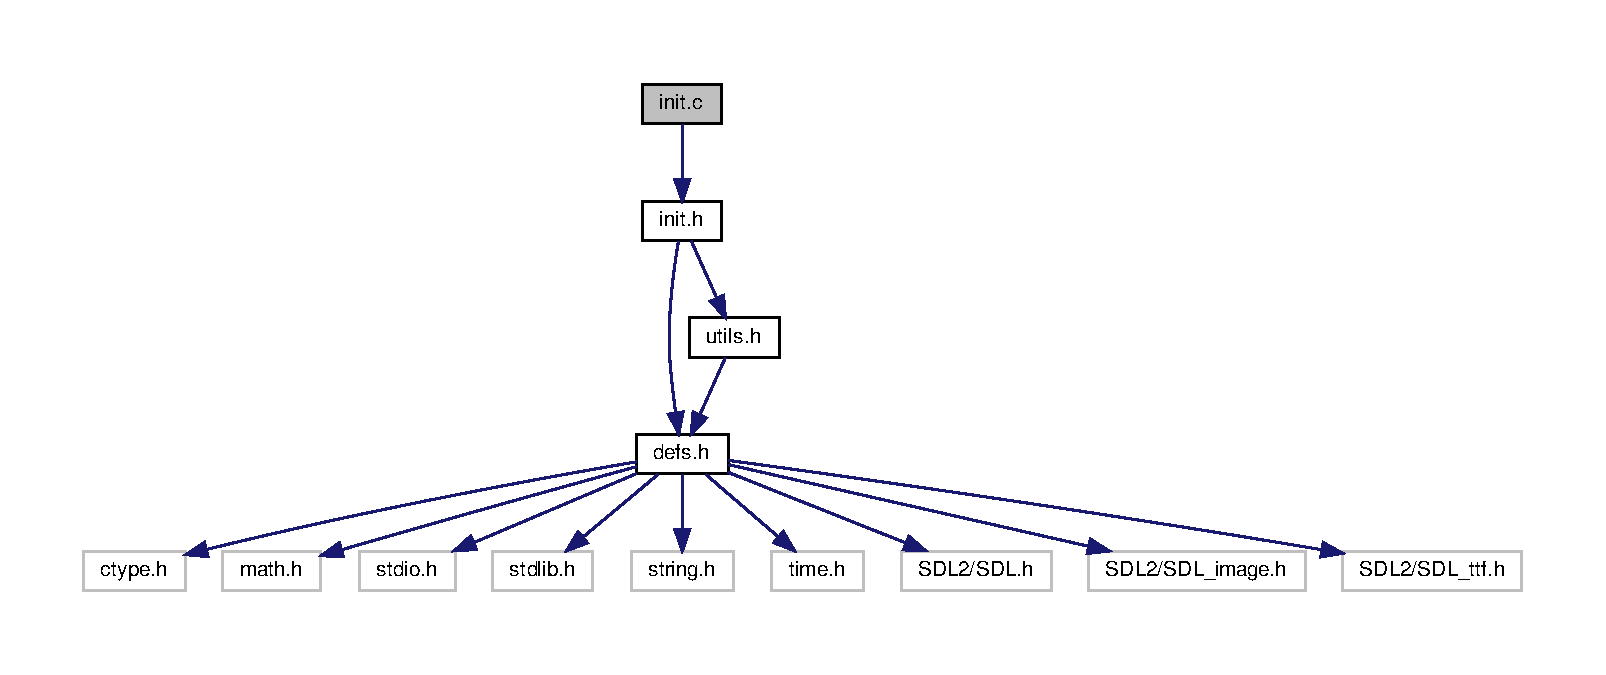
\includegraphics[width=350pt]{init_8c__incl}
\end{center}
\end{figure}
\subsection*{Functions}
\begin{DoxyCompactItemize}
\item 
void \hyperlink{init_8c_a427bf0e70445f92f07adb6512985699d}{Init\+S\+DL} (void)
\begin{DoxyCompactList}\small\item\em 프로그램 수행에 필요한 초기화 과정 수행 \end{DoxyCompactList}\item 
void \hyperlink{init_8c_a82fb88870e950b4d0b484e2744d6b064}{Init\+T\+TF} (void)
\begin{DoxyCompactList}\small\item\em T\+T\+F폰트 사용을 위한 초기화 과정 수행 \end{DoxyCompactList}\item 
void \hyperlink{init_8c_aa2128129f94d9519cfc62de7e308bac7}{Quit\+S\+DL} (int flag)
\begin{DoxyCompactList}\small\item\em 프로그램 종료에 필요한 루틴을 수행하고 프로그램 종료 \end{DoxyCompactList}\item 
void \hyperlink{init_8c_a6ba0c53f3cc9980ebe30a2286632bb45}{Quit\+T\+TF} (void)
\begin{DoxyCompactList}\small\item\em 연 폰트 파일을 닫고 T\+TF 엔진 종료 \end{DoxyCompactList}\item 
void \hyperlink{init_8c_a0a26d5779d3a2a2c898c3f52b74ddf3a}{Init\+Memory\+Set} (void)
\begin{DoxyCompactList}\small\item\em 모든 전역 변수의 메모리 내용 0으로 초기화 \end{DoxyCompactList}\item 
void \hyperlink{init_8c_ab233da79a00de5b6a0752c031b1f9855}{Init\+Score\+Board} (void)
\begin{DoxyCompactList}\small\item\em 스코어보드 초기화(글씨 색깔, 위치) \end{DoxyCompactList}\item 
void \hyperlink{init_8c_a068fc32638e272bb7c61516d6efe4b9e}{Init\+Player} (void)
\begin{DoxyCompactList}\small\item\em 플레이어 초기화 (텍스쳐 불러오기, 위치 설정, 체력 1로 설정) \end{DoxyCompactList}\item 
void \hyperlink{init_8c_a30c1a22616a4bc3d87ab7197913e62d6}{Init\+Bullet} (void)
\begin{DoxyCompactList}\small\item\em 총알 초기화 (텍스쳐 불러오기, 랜덤 위치에 소환, 총알-\/주인공 간 각도계산) \end{DoxyCompactList}\item 
void \hyperlink{init_8c_ac20fccf3f37ac898a607e7ca2aae7081}{Init\+Game\+Over} (void)
\begin{DoxyCompactList}\small\item\em 게임오버 화면 초기화 (텍스쳐, 위치) \end{DoxyCompactList}\end{DoxyCompactItemize}


\subsection{Detailed Description}
무한 루프 진입 전 객체 및 S\+DL 요소 초기화를 위한 함수 정의 

\begin{DoxyAuthor}{Author}
이성재 (\href{mailto:seongjae.lee.1118@gmail.com}{\tt seongjae.\+lee.\+1118@gmail.\+com}) 
\end{DoxyAuthor}


\subsection{Function Documentation}
\mbox{\Hypertarget{init_8c_a30c1a22616a4bc3d87ab7197913e62d6}\label{init_8c_a30c1a22616a4bc3d87ab7197913e62d6}} 
\index{init.\+c@{init.\+c}!Init\+Bullet@{Init\+Bullet}}
\index{Init\+Bullet@{Init\+Bullet}!init.\+c@{init.\+c}}
\subsubsection{\texorpdfstring{Init\+Bullet()}{InitBullet()}}
{\footnotesize\ttfamily void Init\+Bullet (\begin{DoxyParamCaption}\item[{void}]{ }\end{DoxyParamCaption})}



총알 초기화 (텍스쳐 불러오기, 랜덤 위치에 소환, 총알-\/주인공 간 각도계산) 

\begin{DoxyReturn}{Returns}
리턴 값 없음 
\end{DoxyReturn}
\mbox{\Hypertarget{init_8c_ac20fccf3f37ac898a607e7ca2aae7081}\label{init_8c_ac20fccf3f37ac898a607e7ca2aae7081}} 
\index{init.\+c@{init.\+c}!Init\+Game\+Over@{Init\+Game\+Over}}
\index{Init\+Game\+Over@{Init\+Game\+Over}!init.\+c@{init.\+c}}
\subsubsection{\texorpdfstring{Init\+Game\+Over()}{InitGameOver()}}
{\footnotesize\ttfamily void Init\+Game\+Over (\begin{DoxyParamCaption}\item[{void}]{ }\end{DoxyParamCaption})}



게임오버 화면 초기화 (텍스쳐, 위치) 

\begin{DoxyReturn}{Returns}
리턴 값 없음 
\end{DoxyReturn}
\mbox{\Hypertarget{init_8c_a0a26d5779d3a2a2c898c3f52b74ddf3a}\label{init_8c_a0a26d5779d3a2a2c898c3f52b74ddf3a}} 
\index{init.\+c@{init.\+c}!Init\+Memory\+Set@{Init\+Memory\+Set}}
\index{Init\+Memory\+Set@{Init\+Memory\+Set}!init.\+c@{init.\+c}}
\subsubsection{\texorpdfstring{Init\+Memory\+Set()}{InitMemorySet()}}
{\footnotesize\ttfamily void Init\+Memory\+Set (\begin{DoxyParamCaption}\item[{void}]{ }\end{DoxyParamCaption})}



모든 전역 변수의 메모리 내용 0으로 초기화 

\begin{DoxyReturn}{Returns}
리턴 값 없음 
\end{DoxyReturn}
\mbox{\Hypertarget{init_8c_a068fc32638e272bb7c61516d6efe4b9e}\label{init_8c_a068fc32638e272bb7c61516d6efe4b9e}} 
\index{init.\+c@{init.\+c}!Init\+Player@{Init\+Player}}
\index{Init\+Player@{Init\+Player}!init.\+c@{init.\+c}}
\subsubsection{\texorpdfstring{Init\+Player()}{InitPlayer()}}
{\footnotesize\ttfamily void Init\+Player (\begin{DoxyParamCaption}\item[{void}]{ }\end{DoxyParamCaption})}



플레이어 초기화 (텍스쳐 불러오기, 위치 설정, 체력 1로 설정) 

\begin{DoxyReturn}{Returns}
리턴 값 없음 
\end{DoxyReturn}
\mbox{\Hypertarget{init_8c_ab233da79a00de5b6a0752c031b1f9855}\label{init_8c_ab233da79a00de5b6a0752c031b1f9855}} 
\index{init.\+c@{init.\+c}!Init\+Score\+Board@{Init\+Score\+Board}}
\index{Init\+Score\+Board@{Init\+Score\+Board}!init.\+c@{init.\+c}}
\subsubsection{\texorpdfstring{Init\+Score\+Board()}{InitScoreBoard()}}
{\footnotesize\ttfamily void Init\+Score\+Board (\begin{DoxyParamCaption}\item[{void}]{ }\end{DoxyParamCaption})}



스코어보드 초기화(글씨 색깔, 위치) 

\begin{DoxyReturn}{Returns}
리턴 값 없음 
\end{DoxyReturn}
\mbox{\Hypertarget{init_8c_a427bf0e70445f92f07adb6512985699d}\label{init_8c_a427bf0e70445f92f07adb6512985699d}} 
\index{init.\+c@{init.\+c}!Init\+S\+DL@{Init\+S\+DL}}
\index{Init\+S\+DL@{Init\+S\+DL}!init.\+c@{init.\+c}}
\subsubsection{\texorpdfstring{Init\+S\+D\+L()}{InitSDL()}}
{\footnotesize\ttfamily void Init\+S\+DL (\begin{DoxyParamCaption}\item[{void}]{ }\end{DoxyParamCaption})}



프로그램 수행에 필요한 초기화 과정 수행 

\begin{DoxyReturn}{Returns}
리턴 값 없음 
\end{DoxyReturn}
\mbox{\Hypertarget{init_8c_a82fb88870e950b4d0b484e2744d6b064}\label{init_8c_a82fb88870e950b4d0b484e2744d6b064}} 
\index{init.\+c@{init.\+c}!Init\+T\+TF@{Init\+T\+TF}}
\index{Init\+T\+TF@{Init\+T\+TF}!init.\+c@{init.\+c}}
\subsubsection{\texorpdfstring{Init\+T\+T\+F()}{InitTTF()}}
{\footnotesize\ttfamily void Init\+T\+TF (\begin{DoxyParamCaption}\item[{void}]{ }\end{DoxyParamCaption})}



T\+T\+F폰트 사용을 위한 초기화 과정 수행 

\begin{DoxyReturn}{Returns}
리턴 값 없음 
\end{DoxyReturn}
\mbox{\Hypertarget{init_8c_aa2128129f94d9519cfc62de7e308bac7}\label{init_8c_aa2128129f94d9519cfc62de7e308bac7}} 
\index{init.\+c@{init.\+c}!Quit\+S\+DL@{Quit\+S\+DL}}
\index{Quit\+S\+DL@{Quit\+S\+DL}!init.\+c@{init.\+c}}
\subsubsection{\texorpdfstring{Quit\+S\+D\+L()}{QuitSDL()}}
{\footnotesize\ttfamily void Quit\+S\+DL (\begin{DoxyParamCaption}\item[{int}]{flag }\end{DoxyParamCaption})}



프로그램 종료에 필요한 루틴을 수행하고 프로그램 종료 


\begin{DoxyParams}{Parameters}
{\em flag} & 메인 함수에 넘겨줄 프로그램 리턴값\\
\hline
\end{DoxyParams}
\begin{DoxyReturn}{Returns}
리턴 값 없음 
\end{DoxyReturn}
\mbox{\Hypertarget{init_8c_a6ba0c53f3cc9980ebe30a2286632bb45}\label{init_8c_a6ba0c53f3cc9980ebe30a2286632bb45}} 
\index{init.\+c@{init.\+c}!Quit\+T\+TF@{Quit\+T\+TF}}
\index{Quit\+T\+TF@{Quit\+T\+TF}!init.\+c@{init.\+c}}
\subsubsection{\texorpdfstring{Quit\+T\+T\+F()}{QuitTTF()}}
{\footnotesize\ttfamily void Quit\+T\+TF (\begin{DoxyParamCaption}\item[{void}]{ }\end{DoxyParamCaption})}



연 폰트 파일을 닫고 T\+TF 엔진 종료 

\begin{DoxyReturn}{Returns}
리턴 값 없음 
\end{DoxyReturn}

\hypertarget{init_8h}{}\section{init.\+h File Reference}
\label{init_8h}\index{init.\+h@{init.\+h}}


무한 루프 진입 전 객체 및 S\+DL 요소 초기화를 위한 함수 선언  


{\ttfamily \#include \char`\"{}defs.\+h\char`\"{}}\newline
{\ttfamily \#include \char`\"{}utils.\+h\char`\"{}}\newline
Include dependency graph for init.\+h\+:
\nopagebreak
\begin{figure}[H]
\begin{center}
\leavevmode
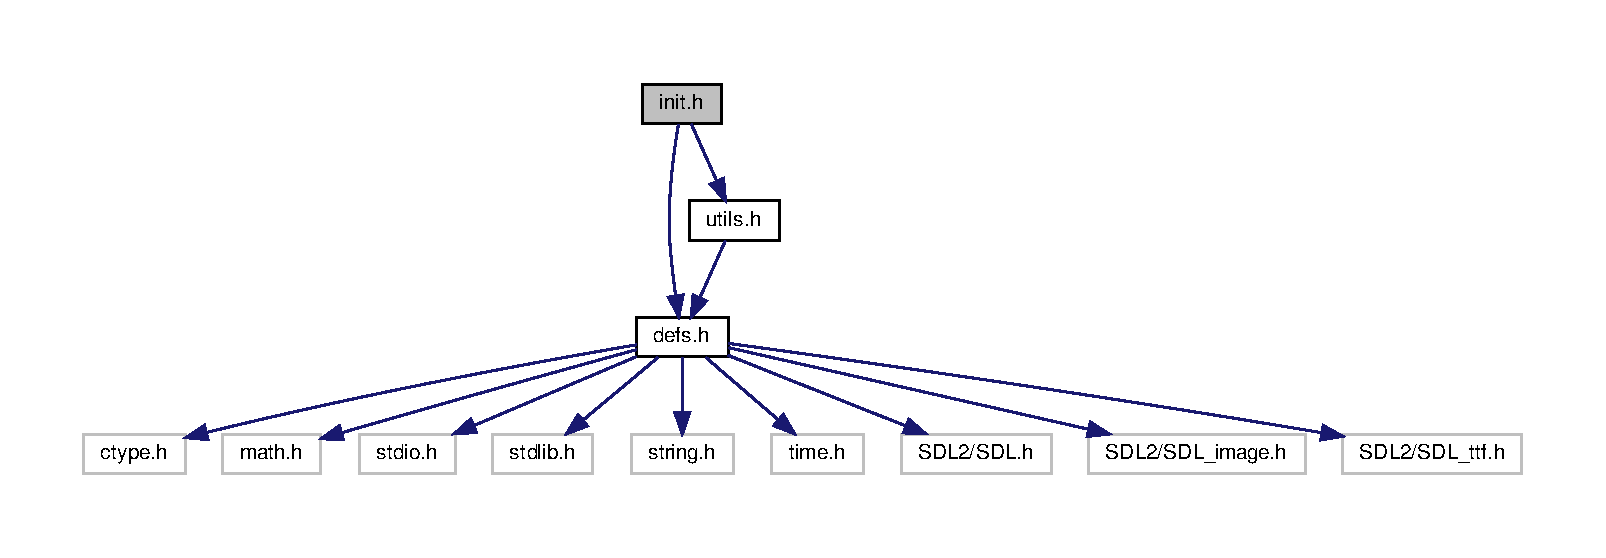
\includegraphics[width=350pt]{init_8h__incl}
\end{center}
\end{figure}
This graph shows which files directly or indirectly include this file\+:
\nopagebreak
\begin{figure}[H]
\begin{center}
\leavevmode
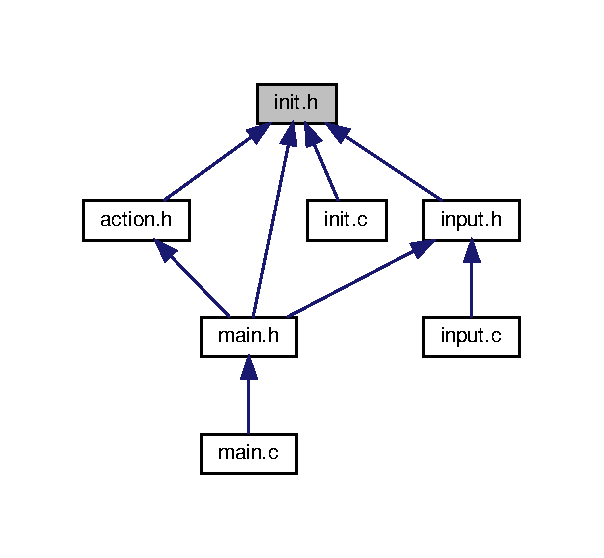
\includegraphics[width=290pt]{init_8h__dep__incl}
\end{center}
\end{figure}
\subsection*{Functions}
\begin{DoxyCompactItemize}
\item 
void \hyperlink{init_8h_a427bf0e70445f92f07adb6512985699d}{Init\+S\+DL} (void)
\begin{DoxyCompactList}\small\item\em 프로그램 수행에 필요한 초기화 과정 수행 \end{DoxyCompactList}\item 
void \hyperlink{init_8h_a82fb88870e950b4d0b484e2744d6b064}{Init\+T\+TF} (void)
\begin{DoxyCompactList}\small\item\em T\+T\+F폰트 사용을 위한 초기화 과정 수행 \end{DoxyCompactList}\item 
void \hyperlink{init_8h_aa2128129f94d9519cfc62de7e308bac7}{Quit\+S\+DL} (int flag)
\begin{DoxyCompactList}\small\item\em 프로그램 종료에 필요한 루틴을 수행하고 프로그램 종료 \end{DoxyCompactList}\item 
void \hyperlink{init_8h_a6ba0c53f3cc9980ebe30a2286632bb45}{Quit\+T\+TF} (void)
\begin{DoxyCompactList}\small\item\em 연 폰트 파일을 닫고 T\+TF 엔진 종료 \end{DoxyCompactList}\item 
void \hyperlink{init_8h_a0a26d5779d3a2a2c898c3f52b74ddf3a}{Init\+Memory\+Set} (void)
\begin{DoxyCompactList}\small\item\em 모든 전역 변수의 메모리 내용 0으로 초기화 \end{DoxyCompactList}\item 
void \hyperlink{init_8h_ab233da79a00de5b6a0752c031b1f9855}{Init\+Score\+Board} (void)
\begin{DoxyCompactList}\small\item\em 스코어보드 초기화(글씨 색깔, 위치) \end{DoxyCompactList}\item 
void \hyperlink{init_8h_a068fc32638e272bb7c61516d6efe4b9e}{Init\+Player} (void)
\begin{DoxyCompactList}\small\item\em 플레이어 초기화 (텍스쳐 불러오기, 위치 설정, 체력 1로 설정) \end{DoxyCompactList}\item 
void \hyperlink{init_8h_a30c1a22616a4bc3d87ab7197913e62d6}{Init\+Bullet} (void)
\begin{DoxyCompactList}\small\item\em 총알 초기화 (텍스쳐 불러오기, 랜덤 위치에 소환, 총알-\/주인공 간 각도계산) \end{DoxyCompactList}\item 
void \hyperlink{init_8h_ac20fccf3f37ac898a607e7ca2aae7081}{Init\+Game\+Over} (void)
\begin{DoxyCompactList}\small\item\em 게임오버 화면 초기화 (텍스쳐, 위치) \end{DoxyCompactList}\end{DoxyCompactItemize}
\subsection*{Variables}
\begin{DoxyCompactItemize}
\item 
\hyperlink{struct_app}{App} \hyperlink{init_8h_a05b5a24325d46227633053ca49de6234}{app}
\item 
\hyperlink{struct_entity}{Entity} \hyperlink{init_8h_aa98761129f4d5e69468dcbdddbd88d9d}{player}
\item 
\hyperlink{struct_entity}{Entity} \hyperlink{init_8h_a3969fcbadddf924ee352d7e232919bf5}{bullet} \mbox{[}\hyperlink{defs_8h_ac2f0ab514de41108a223c4edd49a6dfb}{N\+U\+M\+\_\+\+B\+U\+L\+L\+E\+TS}\mbox{]}
\item 
\hyperlink{struct_entity}{Entity} \hyperlink{init_8h_a30f03aaf13c260e57b759c650c99468e}{game\+\_\+over}
\item 
\hyperlink{struct_text}{Text} \hyperlink{init_8h_afef3fdea043a22bb19f93f3799421010}{score\+\_\+board}
\item 
char \hyperlink{init_8h_ae3c21975ce19d3b28f11d50419e15ab9}{score\+\_\+text} \mbox{[}\hyperlink{defs_8h_aeca034f67218340ecb2261a22c2f3dcd}{B\+U\+F\+S\+I\+ZE}\mbox{]}
\item 
int \hyperlink{init_8h_aef160b7437d94056f1dc59646cd5b87d}{score}
\end{DoxyCompactItemize}


\subsection{Detailed Description}
무한 루프 진입 전 객체 및 S\+DL 요소 초기화를 위한 함수 선언 

\begin{DoxyAuthor}{Author}
이성재 (\href{mailto:seongjae.lee.1118@gmail.com}{\tt seongjae.\+lee.\+1118@gmail.\+com}) 
\end{DoxyAuthor}


\subsection{Function Documentation}
\mbox{\Hypertarget{init_8h_a30c1a22616a4bc3d87ab7197913e62d6}\label{init_8h_a30c1a22616a4bc3d87ab7197913e62d6}} 
\index{init.\+h@{init.\+h}!Init\+Bullet@{Init\+Bullet}}
\index{Init\+Bullet@{Init\+Bullet}!init.\+h@{init.\+h}}
\subsubsection{\texorpdfstring{Init\+Bullet()}{InitBullet()}}
{\footnotesize\ttfamily void Init\+Bullet (\begin{DoxyParamCaption}\item[{void}]{ }\end{DoxyParamCaption})}



총알 초기화 (텍스쳐 불러오기, 랜덤 위치에 소환, 총알-\/주인공 간 각도계산) 

\begin{DoxyReturn}{Returns}
리턴 값 없음 
\end{DoxyReturn}
\mbox{\Hypertarget{init_8h_ac20fccf3f37ac898a607e7ca2aae7081}\label{init_8h_ac20fccf3f37ac898a607e7ca2aae7081}} 
\index{init.\+h@{init.\+h}!Init\+Game\+Over@{Init\+Game\+Over}}
\index{Init\+Game\+Over@{Init\+Game\+Over}!init.\+h@{init.\+h}}
\subsubsection{\texorpdfstring{Init\+Game\+Over()}{InitGameOver()}}
{\footnotesize\ttfamily void Init\+Game\+Over (\begin{DoxyParamCaption}\item[{void}]{ }\end{DoxyParamCaption})}



게임오버 화면 초기화 (텍스쳐, 위치) 

\begin{DoxyReturn}{Returns}
리턴 값 없음 
\end{DoxyReturn}
\mbox{\Hypertarget{init_8h_a0a26d5779d3a2a2c898c3f52b74ddf3a}\label{init_8h_a0a26d5779d3a2a2c898c3f52b74ddf3a}} 
\index{init.\+h@{init.\+h}!Init\+Memory\+Set@{Init\+Memory\+Set}}
\index{Init\+Memory\+Set@{Init\+Memory\+Set}!init.\+h@{init.\+h}}
\subsubsection{\texorpdfstring{Init\+Memory\+Set()}{InitMemorySet()}}
{\footnotesize\ttfamily void Init\+Memory\+Set (\begin{DoxyParamCaption}\item[{void}]{ }\end{DoxyParamCaption})}



모든 전역 변수의 메모리 내용 0으로 초기화 

\begin{DoxyReturn}{Returns}
리턴 값 없음 
\end{DoxyReturn}
\mbox{\Hypertarget{init_8h_a068fc32638e272bb7c61516d6efe4b9e}\label{init_8h_a068fc32638e272bb7c61516d6efe4b9e}} 
\index{init.\+h@{init.\+h}!Init\+Player@{Init\+Player}}
\index{Init\+Player@{Init\+Player}!init.\+h@{init.\+h}}
\subsubsection{\texorpdfstring{Init\+Player()}{InitPlayer()}}
{\footnotesize\ttfamily void Init\+Player (\begin{DoxyParamCaption}\item[{void}]{ }\end{DoxyParamCaption})}



플레이어 초기화 (텍스쳐 불러오기, 위치 설정, 체력 1로 설정) 

\begin{DoxyReturn}{Returns}
리턴 값 없음 
\end{DoxyReturn}
\mbox{\Hypertarget{init_8h_ab233da79a00de5b6a0752c031b1f9855}\label{init_8h_ab233da79a00de5b6a0752c031b1f9855}} 
\index{init.\+h@{init.\+h}!Init\+Score\+Board@{Init\+Score\+Board}}
\index{Init\+Score\+Board@{Init\+Score\+Board}!init.\+h@{init.\+h}}
\subsubsection{\texorpdfstring{Init\+Score\+Board()}{InitScoreBoard()}}
{\footnotesize\ttfamily void Init\+Score\+Board (\begin{DoxyParamCaption}\item[{void}]{ }\end{DoxyParamCaption})}



스코어보드 초기화(글씨 색깔, 위치) 

\begin{DoxyReturn}{Returns}
리턴 값 없음 
\end{DoxyReturn}
\mbox{\Hypertarget{init_8h_a427bf0e70445f92f07adb6512985699d}\label{init_8h_a427bf0e70445f92f07adb6512985699d}} 
\index{init.\+h@{init.\+h}!Init\+S\+DL@{Init\+S\+DL}}
\index{Init\+S\+DL@{Init\+S\+DL}!init.\+h@{init.\+h}}
\subsubsection{\texorpdfstring{Init\+S\+D\+L()}{InitSDL()}}
{\footnotesize\ttfamily void Init\+S\+DL (\begin{DoxyParamCaption}\item[{void}]{ }\end{DoxyParamCaption})}



프로그램 수행에 필요한 초기화 과정 수행 

\begin{DoxyReturn}{Returns}
리턴 값 없음 
\end{DoxyReturn}
\mbox{\Hypertarget{init_8h_a82fb88870e950b4d0b484e2744d6b064}\label{init_8h_a82fb88870e950b4d0b484e2744d6b064}} 
\index{init.\+h@{init.\+h}!Init\+T\+TF@{Init\+T\+TF}}
\index{Init\+T\+TF@{Init\+T\+TF}!init.\+h@{init.\+h}}
\subsubsection{\texorpdfstring{Init\+T\+T\+F()}{InitTTF()}}
{\footnotesize\ttfamily void Init\+T\+TF (\begin{DoxyParamCaption}\item[{void}]{ }\end{DoxyParamCaption})}



T\+T\+F폰트 사용을 위한 초기화 과정 수행 

\begin{DoxyReturn}{Returns}
리턴 값 없음 
\end{DoxyReturn}
\mbox{\Hypertarget{init_8h_aa2128129f94d9519cfc62de7e308bac7}\label{init_8h_aa2128129f94d9519cfc62de7e308bac7}} 
\index{init.\+h@{init.\+h}!Quit\+S\+DL@{Quit\+S\+DL}}
\index{Quit\+S\+DL@{Quit\+S\+DL}!init.\+h@{init.\+h}}
\subsubsection{\texorpdfstring{Quit\+S\+D\+L()}{QuitSDL()}}
{\footnotesize\ttfamily void Quit\+S\+DL (\begin{DoxyParamCaption}\item[{int}]{flag }\end{DoxyParamCaption})}



프로그램 종료에 필요한 루틴을 수행하고 프로그램 종료 


\begin{DoxyParams}{Parameters}
{\em flag} & 메인 함수에 넘겨줄 프로그램 리턴값\\
\hline
\end{DoxyParams}
\begin{DoxyReturn}{Returns}
리턴 값 없음 
\end{DoxyReturn}
\mbox{\Hypertarget{init_8h_a6ba0c53f3cc9980ebe30a2286632bb45}\label{init_8h_a6ba0c53f3cc9980ebe30a2286632bb45}} 
\index{init.\+h@{init.\+h}!Quit\+T\+TF@{Quit\+T\+TF}}
\index{Quit\+T\+TF@{Quit\+T\+TF}!init.\+h@{init.\+h}}
\subsubsection{\texorpdfstring{Quit\+T\+T\+F()}{QuitTTF()}}
{\footnotesize\ttfamily void Quit\+T\+TF (\begin{DoxyParamCaption}\item[{void}]{ }\end{DoxyParamCaption})}



연 폰트 파일을 닫고 T\+TF 엔진 종료 

\begin{DoxyReturn}{Returns}
리턴 값 없음 
\end{DoxyReturn}


\subsection{Variable Documentation}
\mbox{\Hypertarget{init_8h_a05b5a24325d46227633053ca49de6234}\label{init_8h_a05b5a24325d46227633053ca49de6234}} 
\index{init.\+h@{init.\+h}!app@{app}}
\index{app@{app}!init.\+h@{init.\+h}}
\subsubsection{\texorpdfstring{app}{app}}
{\footnotesize\ttfamily \hyperlink{struct_app}{App} app}

프로그램 전체 단위로 관리하는 전역 객체 모음 \mbox{\Hypertarget{init_8h_a3969fcbadddf924ee352d7e232919bf5}\label{init_8h_a3969fcbadddf924ee352d7e232919bf5}} 
\index{init.\+h@{init.\+h}!bullet@{bullet}}
\index{bullet@{bullet}!init.\+h@{init.\+h}}
\subsubsection{\texorpdfstring{bullet}{bullet}}
{\footnotesize\ttfamily \hyperlink{struct_entity}{Entity} bullet\mbox{[}\hyperlink{defs_8h_ac2f0ab514de41108a223c4edd49a6dfb}{N\+U\+M\+\_\+\+B\+U\+L\+L\+E\+TS}\mbox{]}}

총알의 속성을 설명하는 Entity형 구조체 \mbox{\Hypertarget{init_8h_a30f03aaf13c260e57b759c650c99468e}\label{init_8h_a30f03aaf13c260e57b759c650c99468e}} 
\index{init.\+h@{init.\+h}!game\+\_\+over@{game\+\_\+over}}
\index{game\+\_\+over@{game\+\_\+over}!init.\+h@{init.\+h}}
\subsubsection{\texorpdfstring{game\+\_\+over}{game\_over}}
{\footnotesize\ttfamily \hyperlink{struct_entity}{Entity} game\+\_\+over}

게임오버 화면의 속성을 설명하는 Entity형 구조체 \mbox{\Hypertarget{init_8h_aa98761129f4d5e69468dcbdddbd88d9d}\label{init_8h_aa98761129f4d5e69468dcbdddbd88d9d}} 
\index{init.\+h@{init.\+h}!player@{player}}
\index{player@{player}!init.\+h@{init.\+h}}
\subsubsection{\texorpdfstring{player}{player}}
{\footnotesize\ttfamily \hyperlink{struct_entity}{Entity} player}

주인공의 속성을 설명하는 Entity형 구조체 \mbox{\Hypertarget{init_8h_aef160b7437d94056f1dc59646cd5b87d}\label{init_8h_aef160b7437d94056f1dc59646cd5b87d}} 
\index{init.\+h@{init.\+h}!score@{score}}
\index{score@{score}!init.\+h@{init.\+h}}
\subsubsection{\texorpdfstring{score}{score}}
{\footnotesize\ttfamily int score}

게임 스코어 \mbox{\Hypertarget{init_8h_afef3fdea043a22bb19f93f3799421010}\label{init_8h_afef3fdea043a22bb19f93f3799421010}} 
\index{init.\+h@{init.\+h}!score\+\_\+board@{score\+\_\+board}}
\index{score\+\_\+board@{score\+\_\+board}!init.\+h@{init.\+h}}
\subsubsection{\texorpdfstring{score\+\_\+board}{score\_board}}
{\footnotesize\ttfamily \hyperlink{struct_text}{Text} score\+\_\+board}

우상단 스코어보드 문자열을 설명하는 Text형 구조체 \mbox{\Hypertarget{init_8h_ae3c21975ce19d3b28f11d50419e15ab9}\label{init_8h_ae3c21975ce19d3b28f11d50419e15ab9}} 
\index{init.\+h@{init.\+h}!score\+\_\+text@{score\+\_\+text}}
\index{score\+\_\+text@{score\+\_\+text}!init.\+h@{init.\+h}}
\subsubsection{\texorpdfstring{score\+\_\+text}{score\_text}}
{\footnotesize\ttfamily char score\+\_\+text\mbox{[}\hyperlink{defs_8h_aeca034f67218340ecb2261a22c2f3dcd}{B\+U\+F\+S\+I\+ZE}\mbox{]}}

스코어보드에 출력할 문자열 
\hypertarget{input_8c}{}\section{input.\+c File Reference}
\label{input_8c}\index{input.\+c@{input.\+c}}


키보드 입력 발생 시 처리하는 함수 정의  


{\ttfamily \#include \char`\"{}input.\+h\char`\"{}}\newline
Include dependency graph for input.\+c\+:
\nopagebreak
\begin{figure}[H]
\begin{center}
\leavevmode
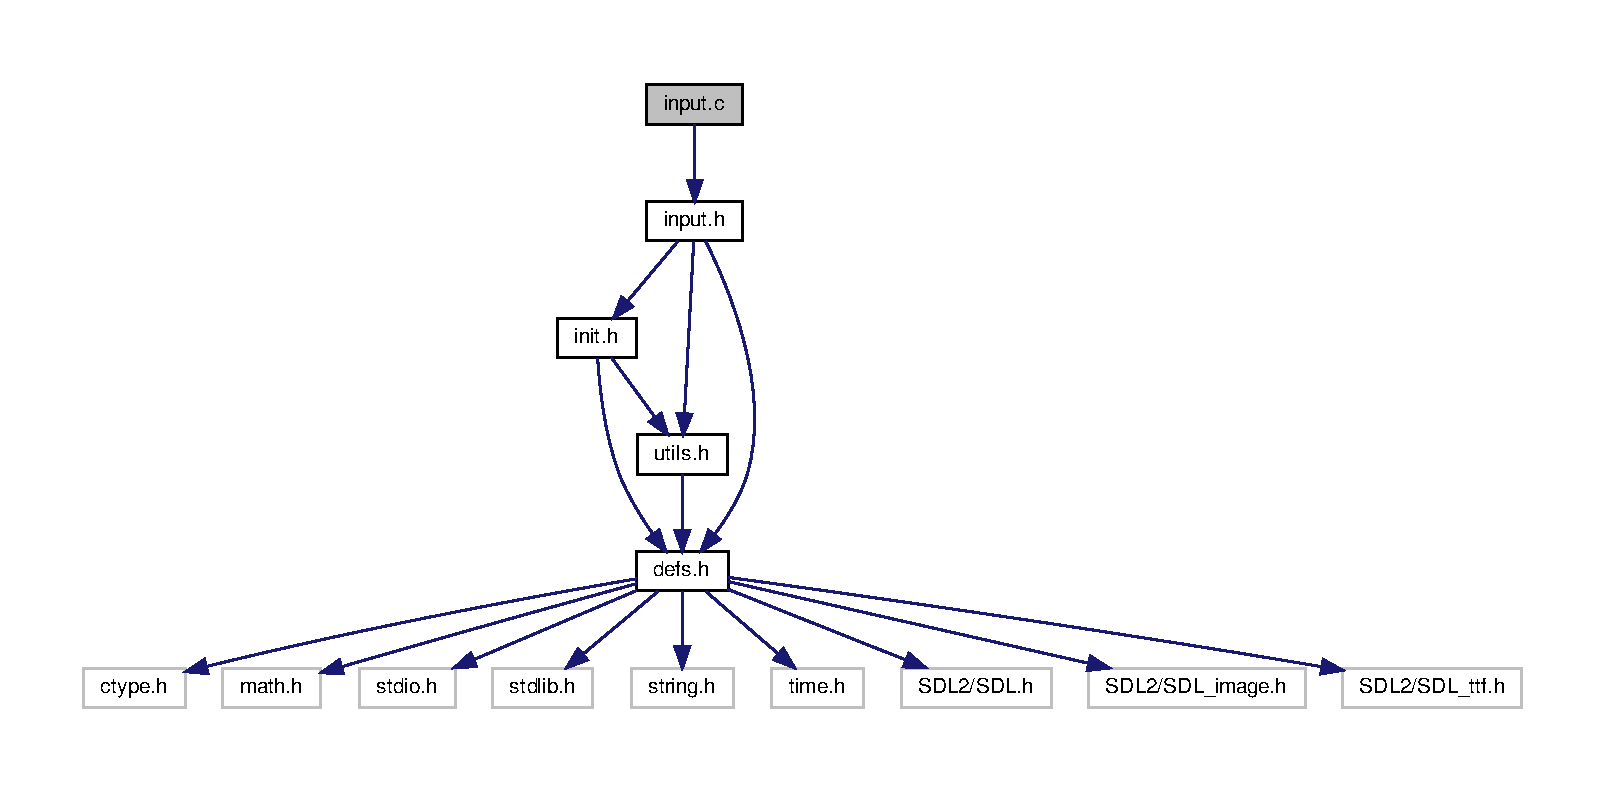
\includegraphics[width=350pt]{input_8c__incl}
\end{center}
\end{figure}
\subsection*{Functions}
\begin{DoxyCompactItemize}
\item 
void \hyperlink{input_8c_a842c28d20fb76863eabd0b7bbbce583d}{Get\+Input} (void)
\begin{DoxyCompactList}\small\item\em 외부 입력을 받아 적절한 동작을 취하도록 한다. \end{DoxyCompactList}\item 
void \hyperlink{input_8c_a760f3d944fc0e0a2c9636d785cd07ca8}{Response\+Key\+Up} (S\+D\+L\+\_\+\+Keyboard\+Event $\ast$event)
\begin{DoxyCompactList}\small\item\em 키보드를 뗐을 때 상태를 기록한다. \end{DoxyCompactList}\item 
void \hyperlink{input_8c_a1b8817382ef71218b5c24982e9320b8a}{Response\+Key\+Down} (S\+D\+L\+\_\+\+Keyboard\+Event $\ast$event)
\begin{DoxyCompactList}\small\item\em 키보드를 눌렀을 때 상태를 기록한다. \end{DoxyCompactList}\end{DoxyCompactItemize}


\subsection{Detailed Description}
키보드 입력 발생 시 처리하는 함수 정의 

\begin{DoxyAuthor}{Author}
이성재 (\href{mailto:seongjae.lee.1118@gmail.com}{\tt seongjae.\+lee.\+1118@gmail.\+com}) 
\end{DoxyAuthor}


\subsection{Function Documentation}
\mbox{\Hypertarget{input_8c_a842c28d20fb76863eabd0b7bbbce583d}\label{input_8c_a842c28d20fb76863eabd0b7bbbce583d}} 
\index{input.\+c@{input.\+c}!Get\+Input@{Get\+Input}}
\index{Get\+Input@{Get\+Input}!input.\+c@{input.\+c}}
\subsubsection{\texorpdfstring{Get\+Input()}{GetInput()}}
{\footnotesize\ttfamily void Get\+Input (\begin{DoxyParamCaption}\item[{void}]{ }\end{DoxyParamCaption})}



외부 입력을 받아 적절한 동작을 취하도록 한다. 

\begin{DoxyReturn}{Returns}
리턴 값 없음 
\end{DoxyReturn}
\mbox{\Hypertarget{input_8c_a1b8817382ef71218b5c24982e9320b8a}\label{input_8c_a1b8817382ef71218b5c24982e9320b8a}} 
\index{input.\+c@{input.\+c}!Response\+Key\+Down@{Response\+Key\+Down}}
\index{Response\+Key\+Down@{Response\+Key\+Down}!input.\+c@{input.\+c}}
\subsubsection{\texorpdfstring{Response\+Key\+Down()}{ResponseKeyDown()}}
{\footnotesize\ttfamily void Response\+Key\+Down (\begin{DoxyParamCaption}\item[{S\+D\+L\+\_\+\+Keyboard\+Event $\ast$}]{event }\end{DoxyParamCaption})}



키보드를 눌렀을 때 상태를 기록한다. 

\begin{DoxyReturn}{Returns}
리턴 값 없음 
\end{DoxyReturn}
\mbox{\Hypertarget{input_8c_a760f3d944fc0e0a2c9636d785cd07ca8}\label{input_8c_a760f3d944fc0e0a2c9636d785cd07ca8}} 
\index{input.\+c@{input.\+c}!Response\+Key\+Up@{Response\+Key\+Up}}
\index{Response\+Key\+Up@{Response\+Key\+Up}!input.\+c@{input.\+c}}
\subsubsection{\texorpdfstring{Response\+Key\+Up()}{ResponseKeyUp()}}
{\footnotesize\ttfamily void Response\+Key\+Up (\begin{DoxyParamCaption}\item[{S\+D\+L\+\_\+\+Keyboard\+Event $\ast$}]{event }\end{DoxyParamCaption})}



키보드를 뗐을 때 상태를 기록한다. 

\begin{DoxyReturn}{Returns}
리턴 값 없음 
\end{DoxyReturn}

\hypertarget{input_8h}{}\section{input.\+h File Reference}
\label{input_8h}\index{input.\+h@{input.\+h}}


키보드 입력 발생 시 처리하는 함수 선언  


{\ttfamily \#include \char`\"{}init.\+h\char`\"{}}\newline
{\ttfamily \#include \char`\"{}defs.\+h\char`\"{}}\newline
{\ttfamily \#include \char`\"{}utils.\+h\char`\"{}}\newline
Include dependency graph for input.\+h\+:
\nopagebreak
\begin{figure}[H]
\begin{center}
\leavevmode
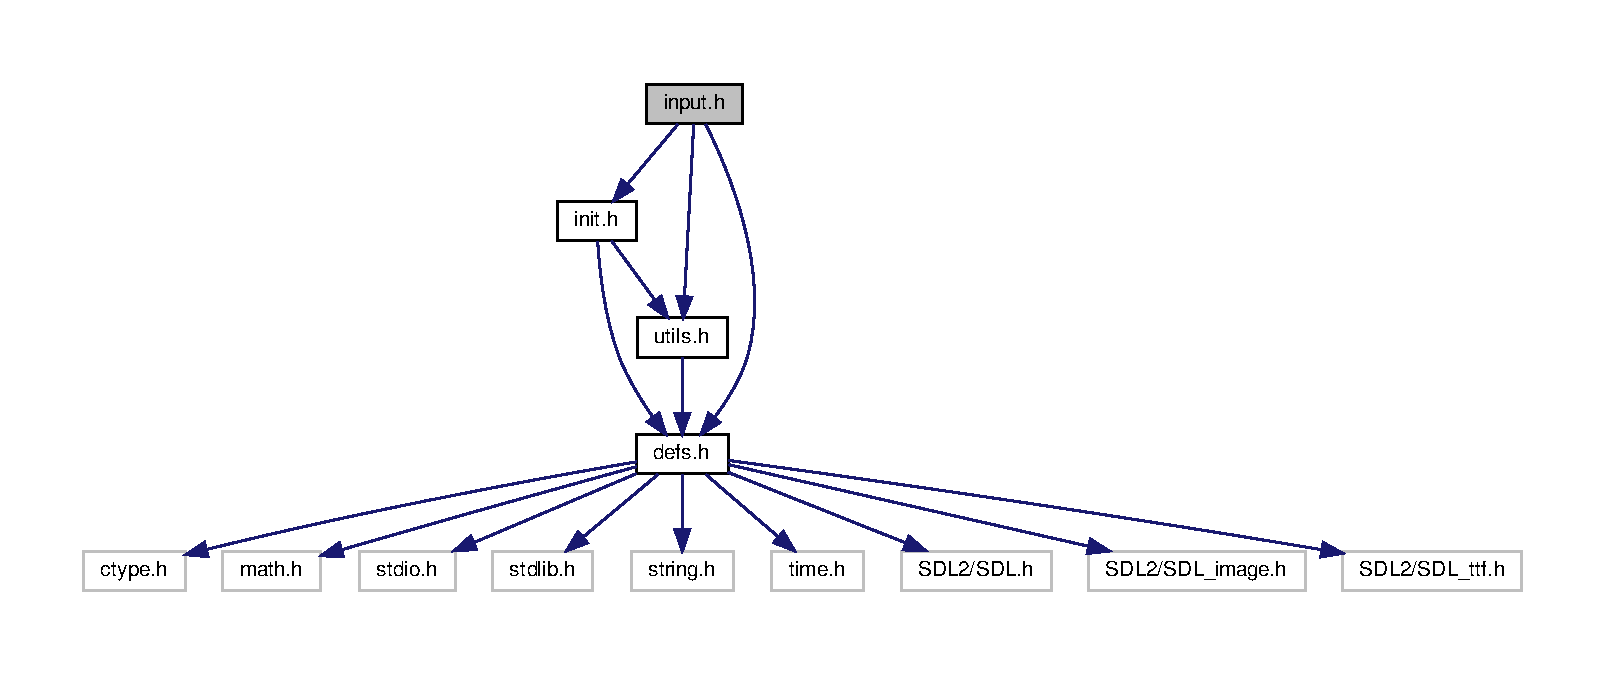
\includegraphics[width=350pt]{input_8h__incl}
\end{center}
\end{figure}
This graph shows which files directly or indirectly include this file\+:
\nopagebreak
\begin{figure}[H]
\begin{center}
\leavevmode
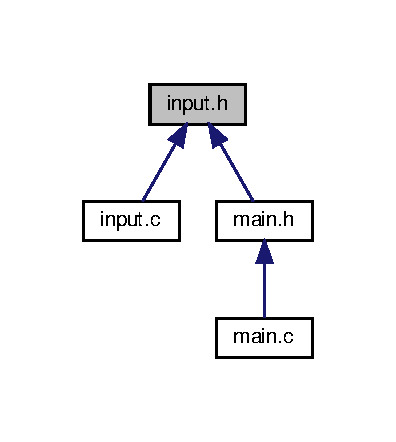
\includegraphics[width=190pt]{input_8h__dep__incl}
\end{center}
\end{figure}
\subsection*{Functions}
\begin{DoxyCompactItemize}
\item 
void \hyperlink{input_8h_a842c28d20fb76863eabd0b7bbbce583d}{Get\+Input} (void)
\begin{DoxyCompactList}\small\item\em 외부 입력을 받아 적절한 동작을 취하도록 한다. \end{DoxyCompactList}\item 
void \hyperlink{input_8h_a760f3d944fc0e0a2c9636d785cd07ca8}{Response\+Key\+Up} (S\+D\+L\+\_\+\+Keyboard\+Event $\ast$event)
\begin{DoxyCompactList}\small\item\em 키보드를 뗐을 때 상태를 기록한다. \end{DoxyCompactList}\item 
void \hyperlink{input_8h_a1b8817382ef71218b5c24982e9320b8a}{Response\+Key\+Down} (S\+D\+L\+\_\+\+Keyboard\+Event $\ast$event)
\begin{DoxyCompactList}\small\item\em 키보드를 눌렀을 때 상태를 기록한다. \end{DoxyCompactList}\end{DoxyCompactItemize}
\subsection*{Variables}
\begin{DoxyCompactItemize}
\item 
\hyperlink{struct_app}{App} \hyperlink{input_8h_a05b5a24325d46227633053ca49de6234}{app}
\item 
\hyperlink{struct_entity}{Entity} \hyperlink{input_8h_aa98761129f4d5e69468dcbdddbd88d9d}{player}
\item 
\hyperlink{struct_entity}{Entity} \hyperlink{input_8h_a3969fcbadddf924ee352d7e232919bf5}{bullet} \mbox{[}\hyperlink{defs_8h_ac2f0ab514de41108a223c4edd49a6dfb}{N\+U\+M\+\_\+\+B\+U\+L\+L\+E\+TS}\mbox{]}
\item 
\hyperlink{struct_entity}{Entity} \hyperlink{input_8h_a30f03aaf13c260e57b759c650c99468e}{game\+\_\+over}
\item 
\hyperlink{struct_text}{Text} \hyperlink{input_8h_afef3fdea043a22bb19f93f3799421010}{score\+\_\+board}
\item 
char \hyperlink{input_8h_ae3c21975ce19d3b28f11d50419e15ab9}{score\+\_\+text} \mbox{[}\hyperlink{defs_8h_aeca034f67218340ecb2261a22c2f3dcd}{B\+U\+F\+S\+I\+ZE}\mbox{]}
\item 
int \hyperlink{input_8h_aef160b7437d94056f1dc59646cd5b87d}{score}
\end{DoxyCompactItemize}


\subsection{Detailed Description}
키보드 입력 발생 시 처리하는 함수 선언 

\begin{DoxyAuthor}{Author}
이성재 (\href{mailto:seongjae.lee.1118@gmail.com}{\tt seongjae.\+lee.\+1118@gmail.\+com}) 
\end{DoxyAuthor}


\subsection{Function Documentation}
\mbox{\Hypertarget{input_8h_a842c28d20fb76863eabd0b7bbbce583d}\label{input_8h_a842c28d20fb76863eabd0b7bbbce583d}} 
\index{input.\+h@{input.\+h}!Get\+Input@{Get\+Input}}
\index{Get\+Input@{Get\+Input}!input.\+h@{input.\+h}}
\subsubsection{\texorpdfstring{Get\+Input()}{GetInput()}}
{\footnotesize\ttfamily void Get\+Input (\begin{DoxyParamCaption}\item[{void}]{ }\end{DoxyParamCaption})}



외부 입력을 받아 적절한 동작을 취하도록 한다. 

\begin{DoxyReturn}{Returns}
리턴 값 없음 
\end{DoxyReturn}
\mbox{\Hypertarget{input_8h_a1b8817382ef71218b5c24982e9320b8a}\label{input_8h_a1b8817382ef71218b5c24982e9320b8a}} 
\index{input.\+h@{input.\+h}!Response\+Key\+Down@{Response\+Key\+Down}}
\index{Response\+Key\+Down@{Response\+Key\+Down}!input.\+h@{input.\+h}}
\subsubsection{\texorpdfstring{Response\+Key\+Down()}{ResponseKeyDown()}}
{\footnotesize\ttfamily void Response\+Key\+Down (\begin{DoxyParamCaption}\item[{S\+D\+L\+\_\+\+Keyboard\+Event $\ast$}]{event }\end{DoxyParamCaption})}



키보드를 눌렀을 때 상태를 기록한다. 

\begin{DoxyReturn}{Returns}
리턴 값 없음 
\end{DoxyReturn}
\mbox{\Hypertarget{input_8h_a760f3d944fc0e0a2c9636d785cd07ca8}\label{input_8h_a760f3d944fc0e0a2c9636d785cd07ca8}} 
\index{input.\+h@{input.\+h}!Response\+Key\+Up@{Response\+Key\+Up}}
\index{Response\+Key\+Up@{Response\+Key\+Up}!input.\+h@{input.\+h}}
\subsubsection{\texorpdfstring{Response\+Key\+Up()}{ResponseKeyUp()}}
{\footnotesize\ttfamily void Response\+Key\+Up (\begin{DoxyParamCaption}\item[{S\+D\+L\+\_\+\+Keyboard\+Event $\ast$}]{event }\end{DoxyParamCaption})}



키보드를 뗐을 때 상태를 기록한다. 

\begin{DoxyReturn}{Returns}
리턴 값 없음 
\end{DoxyReturn}


\subsection{Variable Documentation}
\mbox{\Hypertarget{input_8h_a05b5a24325d46227633053ca49de6234}\label{input_8h_a05b5a24325d46227633053ca49de6234}} 
\index{input.\+h@{input.\+h}!app@{app}}
\index{app@{app}!input.\+h@{input.\+h}}
\subsubsection{\texorpdfstring{app}{app}}
{\footnotesize\ttfamily \hyperlink{struct_app}{App} app}

프로그램 전체 단위로 관리하는 전역 객체 모음 \mbox{\Hypertarget{input_8h_a3969fcbadddf924ee352d7e232919bf5}\label{input_8h_a3969fcbadddf924ee352d7e232919bf5}} 
\index{input.\+h@{input.\+h}!bullet@{bullet}}
\index{bullet@{bullet}!input.\+h@{input.\+h}}
\subsubsection{\texorpdfstring{bullet}{bullet}}
{\footnotesize\ttfamily \hyperlink{struct_entity}{Entity} bullet\mbox{[}\hyperlink{defs_8h_ac2f0ab514de41108a223c4edd49a6dfb}{N\+U\+M\+\_\+\+B\+U\+L\+L\+E\+TS}\mbox{]}}

총알의 속성을 설명하는 Entity형 구조체 \mbox{\Hypertarget{input_8h_a30f03aaf13c260e57b759c650c99468e}\label{input_8h_a30f03aaf13c260e57b759c650c99468e}} 
\index{input.\+h@{input.\+h}!game\+\_\+over@{game\+\_\+over}}
\index{game\+\_\+over@{game\+\_\+over}!input.\+h@{input.\+h}}
\subsubsection{\texorpdfstring{game\+\_\+over}{game\_over}}
{\footnotesize\ttfamily \hyperlink{struct_entity}{Entity} game\+\_\+over}

게임오버 화면의 속성을 설명하는 Entity형 구조체 \mbox{\Hypertarget{input_8h_aa98761129f4d5e69468dcbdddbd88d9d}\label{input_8h_aa98761129f4d5e69468dcbdddbd88d9d}} 
\index{input.\+h@{input.\+h}!player@{player}}
\index{player@{player}!input.\+h@{input.\+h}}
\subsubsection{\texorpdfstring{player}{player}}
{\footnotesize\ttfamily \hyperlink{struct_entity}{Entity} player}

주인공의 속성을 설명하는 Entity형 구조체 \mbox{\Hypertarget{input_8h_aef160b7437d94056f1dc59646cd5b87d}\label{input_8h_aef160b7437d94056f1dc59646cd5b87d}} 
\index{input.\+h@{input.\+h}!score@{score}}
\index{score@{score}!input.\+h@{input.\+h}}
\subsubsection{\texorpdfstring{score}{score}}
{\footnotesize\ttfamily int score}

게임 스코어 \mbox{\Hypertarget{input_8h_afef3fdea043a22bb19f93f3799421010}\label{input_8h_afef3fdea043a22bb19f93f3799421010}} 
\index{input.\+h@{input.\+h}!score\+\_\+board@{score\+\_\+board}}
\index{score\+\_\+board@{score\+\_\+board}!input.\+h@{input.\+h}}
\subsubsection{\texorpdfstring{score\+\_\+board}{score\_board}}
{\footnotesize\ttfamily \hyperlink{struct_text}{Text} score\+\_\+board}

우상단 스코어보드 문자열을 설명하는 Text형 구조체 \mbox{\Hypertarget{input_8h_ae3c21975ce19d3b28f11d50419e15ab9}\label{input_8h_ae3c21975ce19d3b28f11d50419e15ab9}} 
\index{input.\+h@{input.\+h}!score\+\_\+text@{score\+\_\+text}}
\index{score\+\_\+text@{score\+\_\+text}!input.\+h@{input.\+h}}
\subsubsection{\texorpdfstring{score\+\_\+text}{score\_text}}
{\footnotesize\ttfamily char score\+\_\+text\mbox{[}\hyperlink{defs_8h_aeca034f67218340ecb2261a22c2f3dcd}{B\+U\+F\+S\+I\+ZE}\mbox{]}}

스코어보드에 출력할 문자열 
\hypertarget{main_8c}{}\section{main.\+c File Reference}
\label{main_8c}\index{main.\+c@{main.\+c}}


dodger 게임 main 함수를 정의한 소스 파일  


{\ttfamily \#include \char`\"{}main.\+h\char`\"{}}\newline
Include dependency graph for main.\+c\+:
\nopagebreak
\begin{figure}[H]
\begin{center}
\leavevmode
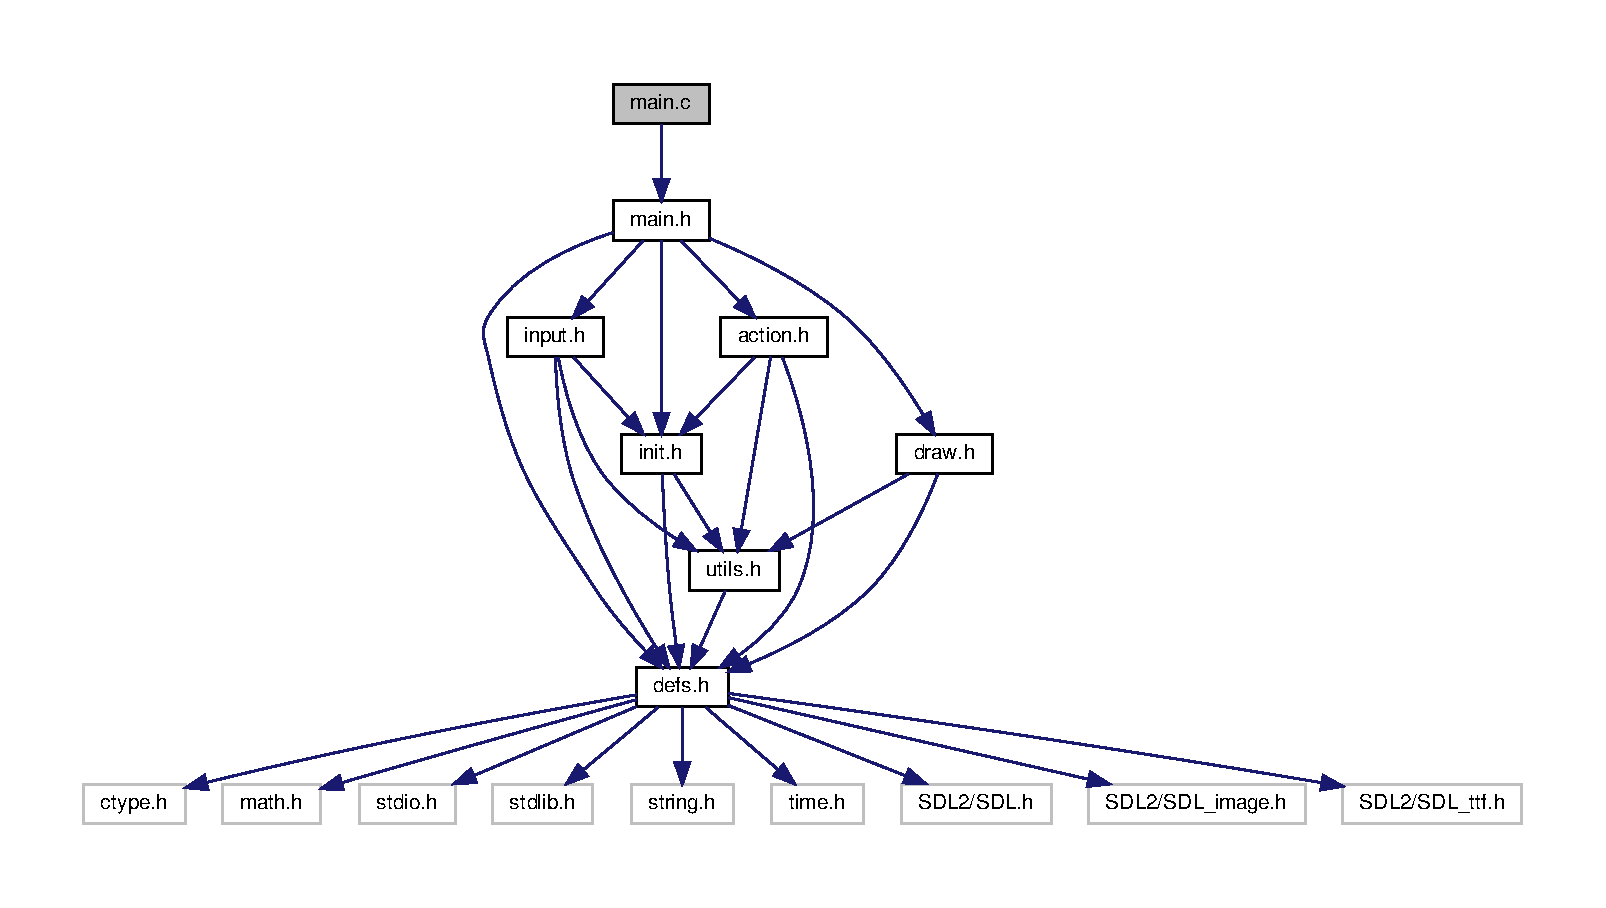
\includegraphics[width=350pt]{main_8c__incl}
\end{center}
\end{figure}
\subsection*{Functions}
\begin{DoxyCompactItemize}
\item 
\mbox{\Hypertarget{main_8c_a840291bc02cba5474a4cb46a9b9566fe}\label{main_8c_a840291bc02cba5474a4cb46a9b9566fe}} 
int {\bfseries main} (void)
\end{DoxyCompactItemize}


\subsection{Detailed Description}
dodger 게임 main 함수를 정의한 소스 파일 

\begin{DoxyAuthor}{Author}
이성재 (\href{mailto:seongjae.lee.1118@gmail.com}{\tt seongjae.\+lee.\+1118@gmail.\+com}) 
\end{DoxyAuthor}

\hypertarget{main_8h}{}\section{main.\+h File Reference}
\label{main_8h}\index{main.\+h@{main.\+h}}


각 모듈 헤더 파일 include 및 전역 변수 선언  


{\ttfamily \#include \char`\"{}defs.\+h\char`\"{}}\newline
{\ttfamily \#include \char`\"{}init.\+h\char`\"{}}\newline
{\ttfamily \#include \char`\"{}input.\+h\char`\"{}}\newline
{\ttfamily \#include \char`\"{}action.\+h\char`\"{}}\newline
{\ttfamily \#include \char`\"{}draw.\+h\char`\"{}}\newline
Include dependency graph for main.\+h\+:
\nopagebreak
\begin{figure}[H]
\begin{center}
\leavevmode
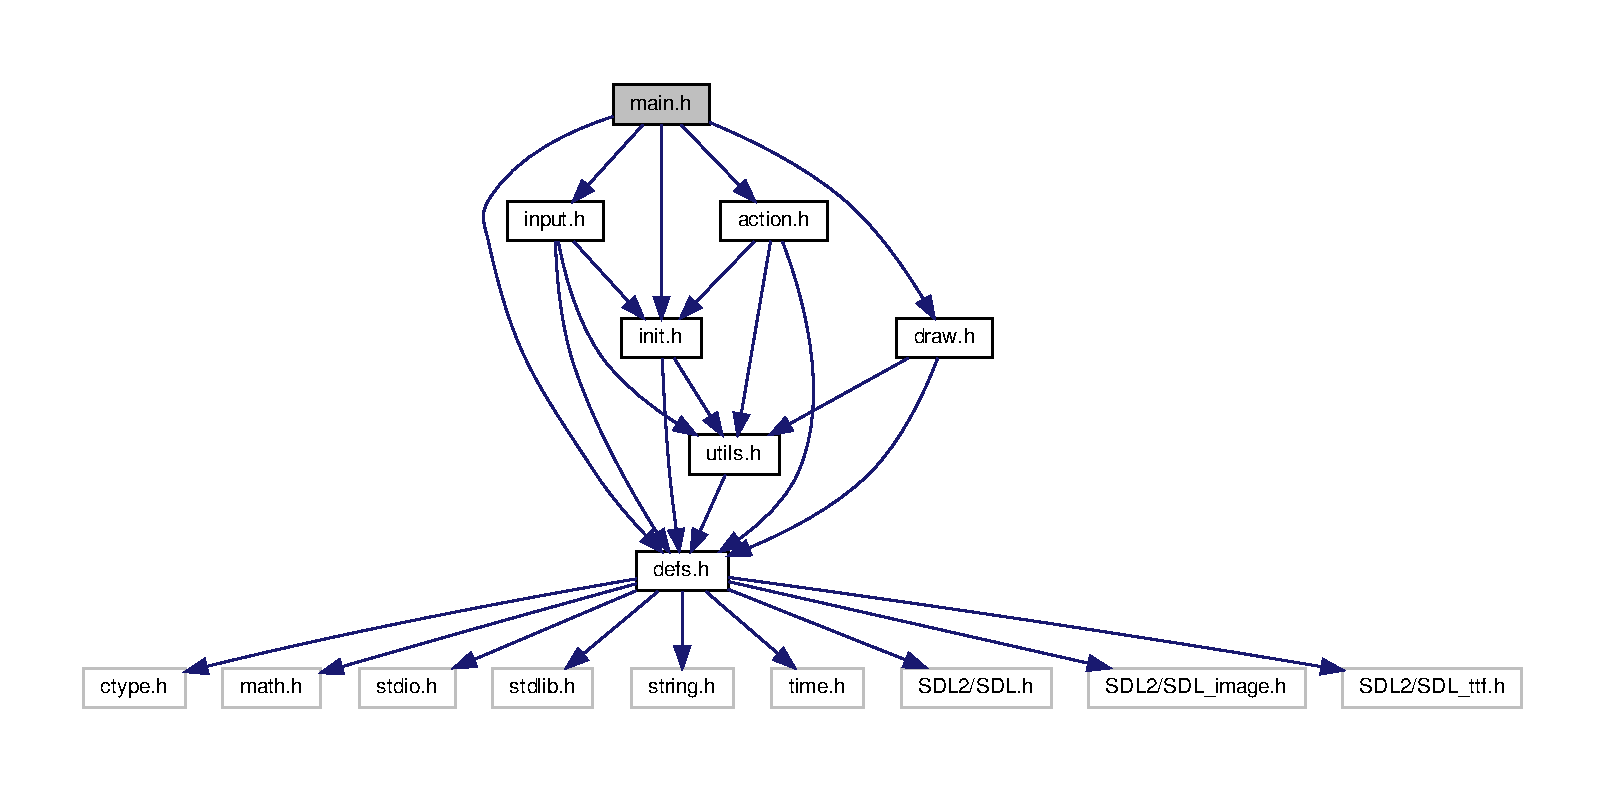
\includegraphics[width=350pt]{main_8h__incl}
\end{center}
\end{figure}
This graph shows which files directly or indirectly include this file\+:
\nopagebreak
\begin{figure}[H]
\begin{center}
\leavevmode
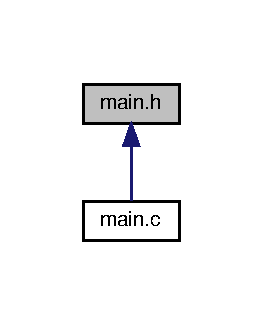
\includegraphics[width=126pt]{main_8h__dep__incl}
\end{center}
\end{figure}
\subsection*{Variables}
\begin{DoxyCompactItemize}
\item 
\hyperlink{struct_app}{App} \hyperlink{main_8h_a05b5a24325d46227633053ca49de6234}{app}
\item 
\hyperlink{struct_entity}{Entity} \hyperlink{main_8h_aa98761129f4d5e69468dcbdddbd88d9d}{player}
\item 
\hyperlink{struct_entity}{Entity} \hyperlink{main_8h_a3969fcbadddf924ee352d7e232919bf5}{bullet} \mbox{[}\hyperlink{defs_8h_ac2f0ab514de41108a223c4edd49a6dfb}{N\+U\+M\+\_\+\+B\+U\+L\+L\+E\+TS}\mbox{]}
\item 
\hyperlink{struct_entity}{Entity} \hyperlink{main_8h_a30f03aaf13c260e57b759c650c99468e}{game\+\_\+over}
\item 
\hyperlink{struct_text}{Text} \hyperlink{main_8h_afef3fdea043a22bb19f93f3799421010}{score\+\_\+board}
\item 
char \hyperlink{main_8h_ae3c21975ce19d3b28f11d50419e15ab9}{score\+\_\+text} \mbox{[}\hyperlink{defs_8h_aeca034f67218340ecb2261a22c2f3dcd}{B\+U\+F\+S\+I\+ZE}\mbox{]}
\item 
int \hyperlink{main_8h_aef160b7437d94056f1dc59646cd5b87d}{score}
\end{DoxyCompactItemize}


\subsection{Detailed Description}
각 모듈 헤더 파일 include 및 전역 변수 선언 

\begin{DoxyAuthor}{Author}
이성재 (\href{mailto:seongjae.lee.1118@gmail.com}{\tt seongjae.\+lee.\+1118@gmail.\+com}) 
\end{DoxyAuthor}


\subsection{Variable Documentation}
\mbox{\Hypertarget{main_8h_a05b5a24325d46227633053ca49de6234}\label{main_8h_a05b5a24325d46227633053ca49de6234}} 
\index{main.\+h@{main.\+h}!app@{app}}
\index{app@{app}!main.\+h@{main.\+h}}
\subsubsection{\texorpdfstring{app}{app}}
{\footnotesize\ttfamily \hyperlink{struct_app}{App} app}

프로그램 전체 단위로 관리하는 전역 객체 모음 \mbox{\Hypertarget{main_8h_a3969fcbadddf924ee352d7e232919bf5}\label{main_8h_a3969fcbadddf924ee352d7e232919bf5}} 
\index{main.\+h@{main.\+h}!bullet@{bullet}}
\index{bullet@{bullet}!main.\+h@{main.\+h}}
\subsubsection{\texorpdfstring{bullet}{bullet}}
{\footnotesize\ttfamily \hyperlink{struct_entity}{Entity} bullet\mbox{[}\hyperlink{defs_8h_ac2f0ab514de41108a223c4edd49a6dfb}{N\+U\+M\+\_\+\+B\+U\+L\+L\+E\+TS}\mbox{]}}

총알의 속성을 설명하는 Entity형 구조체 \mbox{\Hypertarget{main_8h_a30f03aaf13c260e57b759c650c99468e}\label{main_8h_a30f03aaf13c260e57b759c650c99468e}} 
\index{main.\+h@{main.\+h}!game\+\_\+over@{game\+\_\+over}}
\index{game\+\_\+over@{game\+\_\+over}!main.\+h@{main.\+h}}
\subsubsection{\texorpdfstring{game\+\_\+over}{game\_over}}
{\footnotesize\ttfamily \hyperlink{struct_entity}{Entity} game\+\_\+over}

게임오버 화면의 속성을 설명하는 Entity형 구조체 \mbox{\Hypertarget{main_8h_aa98761129f4d5e69468dcbdddbd88d9d}\label{main_8h_aa98761129f4d5e69468dcbdddbd88d9d}} 
\index{main.\+h@{main.\+h}!player@{player}}
\index{player@{player}!main.\+h@{main.\+h}}
\subsubsection{\texorpdfstring{player}{player}}
{\footnotesize\ttfamily \hyperlink{struct_entity}{Entity} player}

주인공의 속성을 설명하는 Entity형 구조체 \mbox{\Hypertarget{main_8h_aef160b7437d94056f1dc59646cd5b87d}\label{main_8h_aef160b7437d94056f1dc59646cd5b87d}} 
\index{main.\+h@{main.\+h}!score@{score}}
\index{score@{score}!main.\+h@{main.\+h}}
\subsubsection{\texorpdfstring{score}{score}}
{\footnotesize\ttfamily int score}

게임 스코어 \mbox{\Hypertarget{main_8h_afef3fdea043a22bb19f93f3799421010}\label{main_8h_afef3fdea043a22bb19f93f3799421010}} 
\index{main.\+h@{main.\+h}!score\+\_\+board@{score\+\_\+board}}
\index{score\+\_\+board@{score\+\_\+board}!main.\+h@{main.\+h}}
\subsubsection{\texorpdfstring{score\+\_\+board}{score\_board}}
{\footnotesize\ttfamily \hyperlink{struct_text}{Text} score\+\_\+board}

우상단 스코어보드 문자열을 설명하는 Text형 구조체 \mbox{\Hypertarget{main_8h_ae3c21975ce19d3b28f11d50419e15ab9}\label{main_8h_ae3c21975ce19d3b28f11d50419e15ab9}} 
\index{main.\+h@{main.\+h}!score\+\_\+text@{score\+\_\+text}}
\index{score\+\_\+text@{score\+\_\+text}!main.\+h@{main.\+h}}
\subsubsection{\texorpdfstring{score\+\_\+text}{score\_text}}
{\footnotesize\ttfamily char score\+\_\+text\mbox{[}\hyperlink{defs_8h_aeca034f67218340ecb2261a22c2f3dcd}{B\+U\+F\+S\+I\+ZE}\mbox{]}}

스코어보드에 출력할 문자열 
\hypertarget{utils_8c}{}\section{utils.\+c File Reference}
\label{utils_8c}\index{utils.\+c@{utils.\+c}}


액션 수행에 필요한 부가적 계산을 수행하는 함수 정의  


{\ttfamily \#include \char`\"{}utils.\+h\char`\"{}}\newline
Include dependency graph for utils.\+c\+:
\nopagebreak
\begin{figure}[H]
\begin{center}
\leavevmode
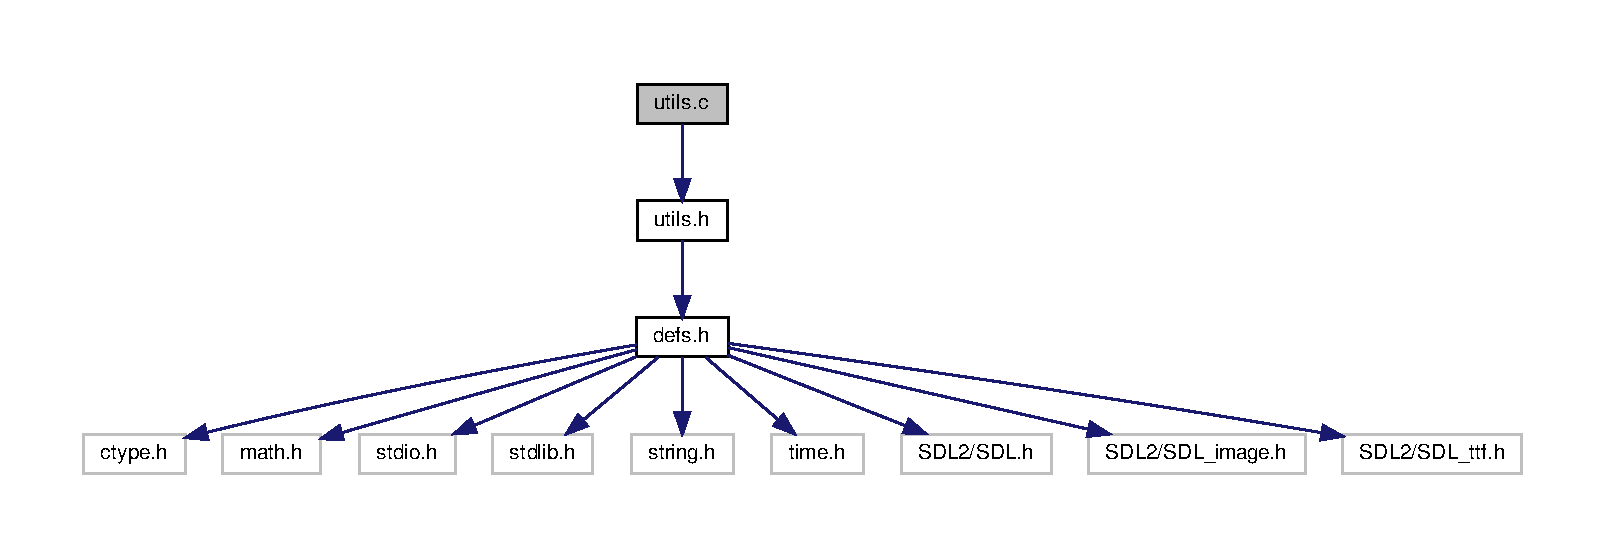
\includegraphics[width=350pt]{utils_8c__incl}
\end{center}
\end{figure}
\subsection*{Functions}
\begin{DoxyCompactItemize}
\item 
int \hyperlink{utils_8c_a53db3177844e1195be84da6b045d19cb}{Check\+Collision\+Wall} (\hyperlink{struct_entity}{Entity} $\ast$object)
\begin{DoxyCompactList}\small\item\em 주인공 혹은 총알이 벽 밖으로 넘어갔는지 확인 \end{DoxyCompactList}\item 
int \hyperlink{utils_8c_ad09f6116d9d2c9a447bff3c40b69d29a}{Check\+Collision\+Objects} (\hyperlink{struct_entity}{Entity} $\ast$object\+\_\+a, \hyperlink{struct_entity}{Entity} $\ast$object\+\_\+b)
\begin{DoxyCompactList}\small\item\em 두 \hyperlink{struct_entity}{Entity} 간 충돌 여부를 판단 \end{DoxyCompactList}\item 
void \hyperlink{utils_8c_a5cb63b050f48798afe28117861e98271}{Rand\+Spawn\+Bullet} (\hyperlink{struct_entity}{Entity} $\ast$object)
\begin{DoxyCompactList}\small\item\em 좌상, 좌하, 우상, 우하단 중 랜덤한 위치에 총알 소환 후 주인공과의 각도 계산 \end{DoxyCompactList}\item 
int \hyperlink{utils_8c_aff4ea7a61b3342b59e917bcc7dd08500}{Rand\+Int} (int min\+\_\+val, int max\+\_\+val)
\begin{DoxyCompactList}\small\item\em \mbox{[}min\+\_\+val, max\+\_\+val) 사이의 무작위 정수를 리턴 \end{DoxyCompactList}\item 
double \hyperlink{utils_8c_a87d33d8b54bca3955ef58a77d52995eb}{Rand\+Double} (double min\+\_\+val, double max\+\_\+val)
\begin{DoxyCompactList}\small\item\em \mbox{[}min\+\_\+val, max\+\_\+val) 사이의 무작위 실수를 리턴 \end{DoxyCompactList}\end{DoxyCompactItemize}


\subsection{Detailed Description}
액션 수행에 필요한 부가적 계산을 수행하는 함수 정의 

\begin{DoxyAuthor}{Author}
이성재 (\href{mailto:seongjae.lee.1118@gmail.com}{\tt seongjae.\+lee.\+1118@gmail.\+com}) 
\end{DoxyAuthor}


\subsection{Function Documentation}
\mbox{\Hypertarget{utils_8c_ad09f6116d9d2c9a447bff3c40b69d29a}\label{utils_8c_ad09f6116d9d2c9a447bff3c40b69d29a}} 
\index{utils.\+c@{utils.\+c}!Check\+Collision\+Objects@{Check\+Collision\+Objects}}
\index{Check\+Collision\+Objects@{Check\+Collision\+Objects}!utils.\+c@{utils.\+c}}
\subsubsection{\texorpdfstring{Check\+Collision\+Objects()}{CheckCollisionObjects()}}
{\footnotesize\ttfamily int Check\+Collision\+Objects (\begin{DoxyParamCaption}\item[{\hyperlink{struct_entity}{Entity} $\ast$}]{object\+\_\+a,  }\item[{\hyperlink{struct_entity}{Entity} $\ast$}]{object\+\_\+b }\end{DoxyParamCaption})}



두 \hyperlink{struct_entity}{Entity} 간 충돌 여부를 판단 


\begin{DoxyParams}{Parameters}
{\em object\+\_\+a} & 충돌 여부를 판단할 첫 번째 \hyperlink{struct_entity}{Entity} 구조체 \\
\hline
{\em object\+\_\+b} & 충돌 여부를 판단할 두 번째 \hyperlink{struct_entity}{Entity} 구조체\\
\hline
\end{DoxyParams}
\begin{DoxyReturn}{Returns}
충돌했으면 1, 충돌하지 않았으면 0 
\end{DoxyReturn}
\mbox{\Hypertarget{utils_8c_a53db3177844e1195be84da6b045d19cb}\label{utils_8c_a53db3177844e1195be84da6b045d19cb}} 
\index{utils.\+c@{utils.\+c}!Check\+Collision\+Wall@{Check\+Collision\+Wall}}
\index{Check\+Collision\+Wall@{Check\+Collision\+Wall}!utils.\+c@{utils.\+c}}
\subsubsection{\texorpdfstring{Check\+Collision\+Wall()}{CheckCollisionWall()}}
{\footnotesize\ttfamily int Check\+Collision\+Wall (\begin{DoxyParamCaption}\item[{\hyperlink{struct_entity}{Entity} $\ast$}]{object }\end{DoxyParamCaption})}



주인공 혹은 총알이 벽 밖으로 넘어갔는지 확인 


\begin{DoxyParams}{Parameters}
{\em object} & 탐지 대상 Entity형 구조체\\
\hline
\end{DoxyParams}
\begin{DoxyReturn}{Returns}
벽 밖으로 넘어가면 1, 벽 안에 있으면 0 
\end{DoxyReturn}
\mbox{\Hypertarget{utils_8c_a87d33d8b54bca3955ef58a77d52995eb}\label{utils_8c_a87d33d8b54bca3955ef58a77d52995eb}} 
\index{utils.\+c@{utils.\+c}!Rand\+Double@{Rand\+Double}}
\index{Rand\+Double@{Rand\+Double}!utils.\+c@{utils.\+c}}
\subsubsection{\texorpdfstring{Rand\+Double()}{RandDouble()}}
{\footnotesize\ttfamily double Rand\+Double (\begin{DoxyParamCaption}\item[{double}]{min\+\_\+val,  }\item[{double}]{max\+\_\+val }\end{DoxyParamCaption})}



\mbox{[}min\+\_\+val, max\+\_\+val) 사이의 무작위 실수를 리턴 


\begin{DoxyParams}{Parameters}
{\em min\+\_\+val} & 최솟값 \\
\hline
{\em max\+\_\+val} & 최댓값\\
\hline
\end{DoxyParams}
\begin{DoxyReturn}{Returns}
생성된 무작위 실수 
\end{DoxyReturn}
\mbox{\Hypertarget{utils_8c_aff4ea7a61b3342b59e917bcc7dd08500}\label{utils_8c_aff4ea7a61b3342b59e917bcc7dd08500}} 
\index{utils.\+c@{utils.\+c}!Rand\+Int@{Rand\+Int}}
\index{Rand\+Int@{Rand\+Int}!utils.\+c@{utils.\+c}}
\subsubsection{\texorpdfstring{Rand\+Int()}{RandInt()}}
{\footnotesize\ttfamily int Rand\+Int (\begin{DoxyParamCaption}\item[{int}]{min\+\_\+val,  }\item[{int}]{max\+\_\+val }\end{DoxyParamCaption})}



\mbox{[}min\+\_\+val, max\+\_\+val) 사이의 무작위 정수를 리턴 


\begin{DoxyParams}{Parameters}
{\em min\+\_\+val} & 최솟값 \\
\hline
{\em max\+\_\+val} & 최댓값\\
\hline
\end{DoxyParams}
\begin{DoxyReturn}{Returns}
생성된 무작위 정수 
\end{DoxyReturn}
\mbox{\Hypertarget{utils_8c_a5cb63b050f48798afe28117861e98271}\label{utils_8c_a5cb63b050f48798afe28117861e98271}} 
\index{utils.\+c@{utils.\+c}!Rand\+Spawn\+Bullet@{Rand\+Spawn\+Bullet}}
\index{Rand\+Spawn\+Bullet@{Rand\+Spawn\+Bullet}!utils.\+c@{utils.\+c}}
\subsubsection{\texorpdfstring{Rand\+Spawn\+Bullet()}{RandSpawnBullet()}}
{\footnotesize\ttfamily void Rand\+Spawn\+Bullet (\begin{DoxyParamCaption}\item[{\hyperlink{struct_entity}{Entity} $\ast$}]{object }\end{DoxyParamCaption})}



좌상, 좌하, 우상, 우하단 중 랜덤한 위치에 총알 소환 후 주인공과의 각도 계산 


\begin{DoxyParams}{Parameters}
{\em object} & 랜덤 소환할 총알 \hyperlink{struct_entity}{Entity}\\
\hline
\end{DoxyParams}
\begin{DoxyReturn}{Returns}
리턴 값 없음 
\end{DoxyReturn}

\hypertarget{utils_8h}{}\section{utils.\+h File Reference}
\label{utils_8h}\index{utils.\+h@{utils.\+h}}


액션 수행에 필요한 부가적 계산을 수행하는 함수 선언  


{\ttfamily \#include \char`\"{}defs.\+h\char`\"{}}\newline
Include dependency graph for utils.\+h\+:
\nopagebreak
\begin{figure}[H]
\begin{center}
\leavevmode
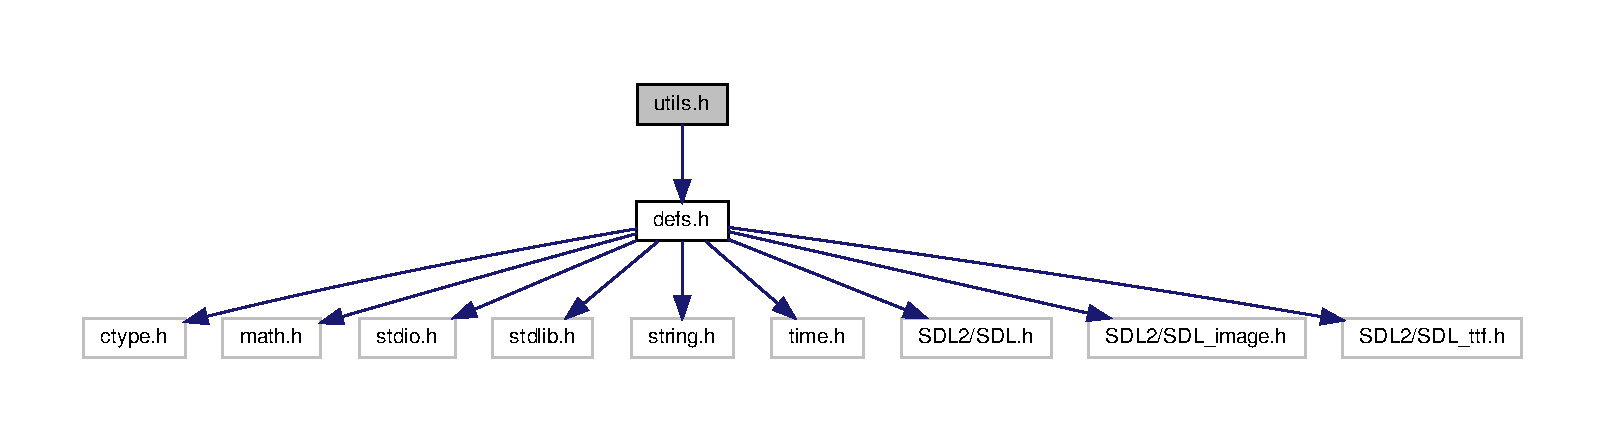
\includegraphics[width=350pt]{utils_8h__incl}
\end{center}
\end{figure}
This graph shows which files directly or indirectly include this file\+:
\nopagebreak
\begin{figure}[H]
\begin{center}
\leavevmode
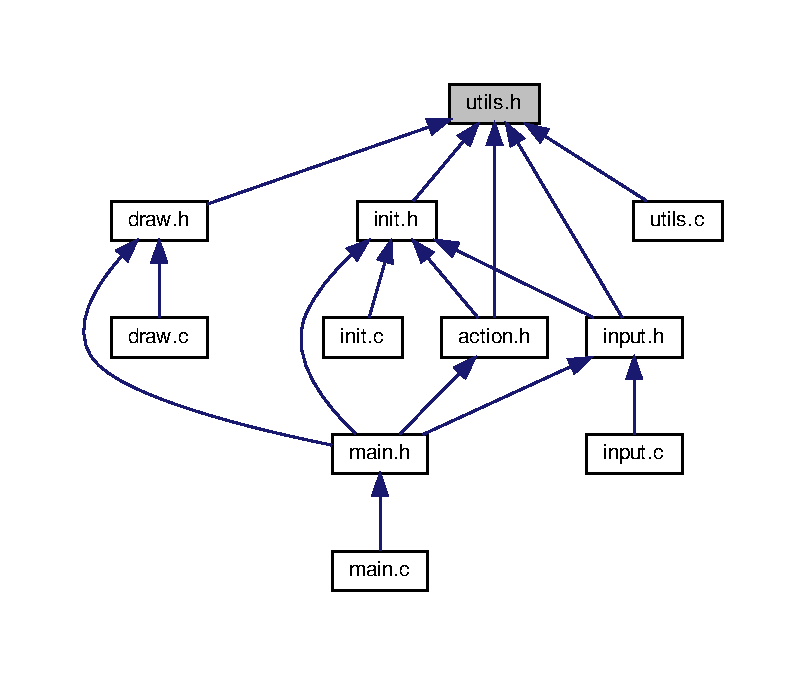
\includegraphics[width=350pt]{utils_8h__dep__incl}
\end{center}
\end{figure}
\subsection*{Functions}
\begin{DoxyCompactItemize}
\item 
int \hyperlink{utils_8h_a53db3177844e1195be84da6b045d19cb}{Check\+Collision\+Wall} (\hyperlink{struct_entity}{Entity} $\ast$object)
\begin{DoxyCompactList}\small\item\em 주인공 혹은 총알이 벽 밖으로 넘어갔는지 확인 \end{DoxyCompactList}\item 
int \hyperlink{utils_8h_ad09f6116d9d2c9a447bff3c40b69d29a}{Check\+Collision\+Objects} (\hyperlink{struct_entity}{Entity} $\ast$object\+\_\+a, \hyperlink{struct_entity}{Entity} $\ast$object\+\_\+b)
\begin{DoxyCompactList}\small\item\em 두 \hyperlink{struct_entity}{Entity} 간 충돌 여부를 판단 \end{DoxyCompactList}\item 
void \hyperlink{utils_8h_a5cb63b050f48798afe28117861e98271}{Rand\+Spawn\+Bullet} (\hyperlink{struct_entity}{Entity} $\ast$object)
\begin{DoxyCompactList}\small\item\em 좌상, 좌하, 우상, 우하단 중 랜덤한 위치에 총알 소환 후 주인공과의 각도 계산 \end{DoxyCompactList}\item 
int \hyperlink{utils_8h_aff4ea7a61b3342b59e917bcc7dd08500}{Rand\+Int} (int min\+\_\+val, int max\+\_\+val)
\begin{DoxyCompactList}\small\item\em \mbox{[}min\+\_\+val, max\+\_\+val) 사이의 무작위 정수를 리턴 \end{DoxyCompactList}\item 
double \hyperlink{utils_8h_a87d33d8b54bca3955ef58a77d52995eb}{Rand\+Double} (double min\+\_\+val, double max\+\_\+val)
\begin{DoxyCompactList}\small\item\em \mbox{[}min\+\_\+val, max\+\_\+val) 사이의 무작위 실수를 리턴 \end{DoxyCompactList}\end{DoxyCompactItemize}
\subsection*{Variables}
\begin{DoxyCompactItemize}
\item 
\hyperlink{struct_app}{App} \hyperlink{utils_8h_a05b5a24325d46227633053ca49de6234}{app}
\item 
\hyperlink{struct_entity}{Entity} \hyperlink{utils_8h_aa98761129f4d5e69468dcbdddbd88d9d}{player}
\item 
\hyperlink{struct_entity}{Entity} \hyperlink{utils_8h_a3969fcbadddf924ee352d7e232919bf5}{bullet} \mbox{[}\hyperlink{defs_8h_ac2f0ab514de41108a223c4edd49a6dfb}{N\+U\+M\+\_\+\+B\+U\+L\+L\+E\+TS}\mbox{]}
\item 
\hyperlink{struct_entity}{Entity} \hyperlink{utils_8h_a30f03aaf13c260e57b759c650c99468e}{game\+\_\+over}
\item 
\hyperlink{struct_text}{Text} \hyperlink{utils_8h_afef3fdea043a22bb19f93f3799421010}{score\+\_\+board}
\item 
char \hyperlink{utils_8h_ae3c21975ce19d3b28f11d50419e15ab9}{score\+\_\+text} \mbox{[}\hyperlink{defs_8h_aeca034f67218340ecb2261a22c2f3dcd}{B\+U\+F\+S\+I\+ZE}\mbox{]}
\item 
int \hyperlink{utils_8h_aef160b7437d94056f1dc59646cd5b87d}{score}
\end{DoxyCompactItemize}


\subsection{Detailed Description}
액션 수행에 필요한 부가적 계산을 수행하는 함수 선언 

\begin{DoxyAuthor}{Author}
이성재 (\href{mailto:seongjae.lee.1118@gmail.com}{\tt seongjae.\+lee.\+1118@gmail.\+com}) 
\end{DoxyAuthor}


\subsection{Function Documentation}
\mbox{\Hypertarget{utils_8h_ad09f6116d9d2c9a447bff3c40b69d29a}\label{utils_8h_ad09f6116d9d2c9a447bff3c40b69d29a}} 
\index{utils.\+h@{utils.\+h}!Check\+Collision\+Objects@{Check\+Collision\+Objects}}
\index{Check\+Collision\+Objects@{Check\+Collision\+Objects}!utils.\+h@{utils.\+h}}
\subsubsection{\texorpdfstring{Check\+Collision\+Objects()}{CheckCollisionObjects()}}
{\footnotesize\ttfamily int Check\+Collision\+Objects (\begin{DoxyParamCaption}\item[{\hyperlink{struct_entity}{Entity} $\ast$}]{object\+\_\+a,  }\item[{\hyperlink{struct_entity}{Entity} $\ast$}]{object\+\_\+b }\end{DoxyParamCaption})}



두 \hyperlink{struct_entity}{Entity} 간 충돌 여부를 판단 


\begin{DoxyParams}{Parameters}
{\em object\+\_\+a} & 충돌 여부를 판단할 첫 번째 \hyperlink{struct_entity}{Entity} 구조체 \\
\hline
{\em object\+\_\+b} & 충돌 여부를 판단할 두 번째 \hyperlink{struct_entity}{Entity} 구조체\\
\hline
\end{DoxyParams}
\begin{DoxyReturn}{Returns}
충돌했으면 1, 충돌하지 않았으면 0 
\end{DoxyReturn}
\mbox{\Hypertarget{utils_8h_a53db3177844e1195be84da6b045d19cb}\label{utils_8h_a53db3177844e1195be84da6b045d19cb}} 
\index{utils.\+h@{utils.\+h}!Check\+Collision\+Wall@{Check\+Collision\+Wall}}
\index{Check\+Collision\+Wall@{Check\+Collision\+Wall}!utils.\+h@{utils.\+h}}
\subsubsection{\texorpdfstring{Check\+Collision\+Wall()}{CheckCollisionWall()}}
{\footnotesize\ttfamily int Check\+Collision\+Wall (\begin{DoxyParamCaption}\item[{\hyperlink{struct_entity}{Entity} $\ast$}]{object }\end{DoxyParamCaption})}



주인공 혹은 총알이 벽 밖으로 넘어갔는지 확인 


\begin{DoxyParams}{Parameters}
{\em object} & 탐지 대상 Entity형 구조체\\
\hline
\end{DoxyParams}
\begin{DoxyReturn}{Returns}
벽 밖으로 넘어가면 1, 벽 안에 있으면 0 
\end{DoxyReturn}
\mbox{\Hypertarget{utils_8h_a87d33d8b54bca3955ef58a77d52995eb}\label{utils_8h_a87d33d8b54bca3955ef58a77d52995eb}} 
\index{utils.\+h@{utils.\+h}!Rand\+Double@{Rand\+Double}}
\index{Rand\+Double@{Rand\+Double}!utils.\+h@{utils.\+h}}
\subsubsection{\texorpdfstring{Rand\+Double()}{RandDouble()}}
{\footnotesize\ttfamily double Rand\+Double (\begin{DoxyParamCaption}\item[{double}]{min\+\_\+val,  }\item[{double}]{max\+\_\+val }\end{DoxyParamCaption})}



\mbox{[}min\+\_\+val, max\+\_\+val) 사이의 무작위 실수를 리턴 


\begin{DoxyParams}{Parameters}
{\em min\+\_\+val} & 최솟값 \\
\hline
{\em max\+\_\+val} & 최댓값\\
\hline
\end{DoxyParams}
\begin{DoxyReturn}{Returns}
생성된 무작위 실수 
\end{DoxyReturn}
\mbox{\Hypertarget{utils_8h_aff4ea7a61b3342b59e917bcc7dd08500}\label{utils_8h_aff4ea7a61b3342b59e917bcc7dd08500}} 
\index{utils.\+h@{utils.\+h}!Rand\+Int@{Rand\+Int}}
\index{Rand\+Int@{Rand\+Int}!utils.\+h@{utils.\+h}}
\subsubsection{\texorpdfstring{Rand\+Int()}{RandInt()}}
{\footnotesize\ttfamily int Rand\+Int (\begin{DoxyParamCaption}\item[{int}]{min\+\_\+val,  }\item[{int}]{max\+\_\+val }\end{DoxyParamCaption})}



\mbox{[}min\+\_\+val, max\+\_\+val) 사이의 무작위 정수를 리턴 


\begin{DoxyParams}{Parameters}
{\em min\+\_\+val} & 최솟값 \\
\hline
{\em max\+\_\+val} & 최댓값\\
\hline
\end{DoxyParams}
\begin{DoxyReturn}{Returns}
생성된 무작위 정수 
\end{DoxyReturn}
\mbox{\Hypertarget{utils_8h_a5cb63b050f48798afe28117861e98271}\label{utils_8h_a5cb63b050f48798afe28117861e98271}} 
\index{utils.\+h@{utils.\+h}!Rand\+Spawn\+Bullet@{Rand\+Spawn\+Bullet}}
\index{Rand\+Spawn\+Bullet@{Rand\+Spawn\+Bullet}!utils.\+h@{utils.\+h}}
\subsubsection{\texorpdfstring{Rand\+Spawn\+Bullet()}{RandSpawnBullet()}}
{\footnotesize\ttfamily void Rand\+Spawn\+Bullet (\begin{DoxyParamCaption}\item[{\hyperlink{struct_entity}{Entity} $\ast$}]{object }\end{DoxyParamCaption})}



좌상, 좌하, 우상, 우하단 중 랜덤한 위치에 총알 소환 후 주인공과의 각도 계산 


\begin{DoxyParams}{Parameters}
{\em object} & 랜덤 소환할 총알 \hyperlink{struct_entity}{Entity}\\
\hline
\end{DoxyParams}
\begin{DoxyReturn}{Returns}
리턴 값 없음 
\end{DoxyReturn}


\subsection{Variable Documentation}
\mbox{\Hypertarget{utils_8h_a05b5a24325d46227633053ca49de6234}\label{utils_8h_a05b5a24325d46227633053ca49de6234}} 
\index{utils.\+h@{utils.\+h}!app@{app}}
\index{app@{app}!utils.\+h@{utils.\+h}}
\subsubsection{\texorpdfstring{app}{app}}
{\footnotesize\ttfamily \hyperlink{struct_app}{App} app}

프로그램 전체 단위로 관리하는 전역 객체 모음 \mbox{\Hypertarget{utils_8h_a3969fcbadddf924ee352d7e232919bf5}\label{utils_8h_a3969fcbadddf924ee352d7e232919bf5}} 
\index{utils.\+h@{utils.\+h}!bullet@{bullet}}
\index{bullet@{bullet}!utils.\+h@{utils.\+h}}
\subsubsection{\texorpdfstring{bullet}{bullet}}
{\footnotesize\ttfamily \hyperlink{struct_entity}{Entity} bullet\mbox{[}\hyperlink{defs_8h_ac2f0ab514de41108a223c4edd49a6dfb}{N\+U\+M\+\_\+\+B\+U\+L\+L\+E\+TS}\mbox{]}}

총알의 속성을 설명하는 Entity형 구조체 \mbox{\Hypertarget{utils_8h_a30f03aaf13c260e57b759c650c99468e}\label{utils_8h_a30f03aaf13c260e57b759c650c99468e}} 
\index{utils.\+h@{utils.\+h}!game\+\_\+over@{game\+\_\+over}}
\index{game\+\_\+over@{game\+\_\+over}!utils.\+h@{utils.\+h}}
\subsubsection{\texorpdfstring{game\+\_\+over}{game\_over}}
{\footnotesize\ttfamily \hyperlink{struct_entity}{Entity} game\+\_\+over}

게임오버 화면의 속성을 설명하는 Entity형 구조체 \mbox{\Hypertarget{utils_8h_aa98761129f4d5e69468dcbdddbd88d9d}\label{utils_8h_aa98761129f4d5e69468dcbdddbd88d9d}} 
\index{utils.\+h@{utils.\+h}!player@{player}}
\index{player@{player}!utils.\+h@{utils.\+h}}
\subsubsection{\texorpdfstring{player}{player}}
{\footnotesize\ttfamily \hyperlink{struct_entity}{Entity} player}

주인공의 속성을 설명하는 Entity형 구조체 \mbox{\Hypertarget{utils_8h_aef160b7437d94056f1dc59646cd5b87d}\label{utils_8h_aef160b7437d94056f1dc59646cd5b87d}} 
\index{utils.\+h@{utils.\+h}!score@{score}}
\index{score@{score}!utils.\+h@{utils.\+h}}
\subsubsection{\texorpdfstring{score}{score}}
{\footnotesize\ttfamily int score}

게임 스코어 \mbox{\Hypertarget{utils_8h_afef3fdea043a22bb19f93f3799421010}\label{utils_8h_afef3fdea043a22bb19f93f3799421010}} 
\index{utils.\+h@{utils.\+h}!score\+\_\+board@{score\+\_\+board}}
\index{score\+\_\+board@{score\+\_\+board}!utils.\+h@{utils.\+h}}
\subsubsection{\texorpdfstring{score\+\_\+board}{score\_board}}
{\footnotesize\ttfamily \hyperlink{struct_text}{Text} score\+\_\+board}

우상단 스코어보드 문자열을 설명하는 Text형 구조체 \mbox{\Hypertarget{utils_8h_ae3c21975ce19d3b28f11d50419e15ab9}\label{utils_8h_ae3c21975ce19d3b28f11d50419e15ab9}} 
\index{utils.\+h@{utils.\+h}!score\+\_\+text@{score\+\_\+text}}
\index{score\+\_\+text@{score\+\_\+text}!utils.\+h@{utils.\+h}}
\subsubsection{\texorpdfstring{score\+\_\+text}{score\_text}}
{\footnotesize\ttfamily char score\+\_\+text\mbox{[}\hyperlink{defs_8h_aeca034f67218340ecb2261a22c2f3dcd}{B\+U\+F\+S\+I\+ZE}\mbox{]}}

스코어보드에 출력할 문자열 
%--- End generated contents ---

% Index
\backmatter
\newpage
\phantomsection
\clearemptydoublepage
\addcontentsline{toc}{chapter}{Index}
\printindex

\end{document}
